\documentclass[11pt,a4paper]{article}

\usepackage[margin=2.5cm,marginparwidth=2cm]{geometry}
\usepackage{fontspec}
\usepackage{microtype}
\usepackage{amsmath,amssymb}
\usepackage{booktabs,tabularx}
\usepackage{graphicx}
\usepackage{enumitem}
\usepackage[authoryear,round]{natbib}
\usepackage[colorinlistoftodos,textsize=small]{todonotes}
\usepackage[hidelinks]{hyperref}

\setlist{itemsep=2pt,topsep=4pt}
\newcommand{\Gz}{G_0}
\newcommand{\Req}{R(G_0)}

\title{From Advisor to Operator:\\Goal Drift through Sub-Task Accumulation in Autonomous Coding Agents}
\author{Giorgio Chiesa\\[2pt]\small PhD course \emph{AI--Human Interaction}, Universit\`a di Torino}
\date{\today}

\begin{document}
\maketitle

\begin{abstract}
Large language models are no longer only consulted: as coding agents such as Claude Code they read
repositories, run commands, edit files and decide what to do next, and the human moves from
\emph{operator} to \emph{approver} or \emph{observer}. We study one risk of this shift: that the
sub-tasks entering a session (broken dependencies, failing tests, instructions found in files, side
requests from the user) accumulate and pull the agent away from its goal. We review the literature,
define \emph{goal drift via sub-task injection} as a counterfactual degradation that separates
sanctioned, necessary and distracting sub-tasks, and test it on DriftBench-mini, twelve coding tasks
with planted sub-tasks, driving Claude Code with two locally hosted open-weight models (1{,}332
episodes). Broken dependencies that the goal relies on reduce goal completion sharply in both models:
from 0.77 to 0.50 and from 0.48 to 0.24 with four of them, beyond a matched-length control. Four side
requests from the user overload only the weaker model, distractors are largely ignored, and four
lightweight harness mitigations do not significantly reduce the loss. A panel of three LLM judges
(Fleiss' $\kappa=0.67$ on the binary off-goal label) finds that off-goal work is mostly legitimate,
distraction is rare and summaries often claim completion while requirements fail. In a
forced-compaction pilot, compaction shifts later effort from the goal towards the user's requests
($+0.13$ off-goal share). A simulated supervisor shows that reviewing or monitoring the agent's
activity catches few failing episodes early, because the failure is incompletion: only checking the
requirements reveals it.
\end{abstract}

\section{Introduction: from advisor to operator}
\label{sec:intro}

For most of their short public history, large language models (LLMs) have been \emph{consultative}
tools. A developer asked a chat assistant how to fix an error, accepted or rejected an inline
completion, and remained the only actor who touched the codebase. The model advised; the human
operated. Every consequential action passed through a human decision, and the cost of a bad
suggestion was bounded by the human's willingness to adopt it.

That arrangement is changing quickly. Coding agents such as Claude Code, OpenHands, Devin, Cursor's
agent mode or Codex receive a goal in natural language, explore a repository, run commands, edit
files, execute tests and decide autonomously what to do next
\citep{yang2024sweagent,wang2024openhands,anthropic2026claudecode}. The capability trend behind
this shift is steep: the length of software tasks, measured in human time, that frontier models
complete with 50\% reliability has been doubling roughly every seven months \citep{kwa2025measuring}.
Adoption is equally fast. Within months of their release, coding agents left traces in an estimated
22--29\% of a large sample of GitHub projects \citep{robbes2026agentic}, and datasets now count
close to a million agent-authored pull requests \citep{li2026aidev}.

In the vocabulary of \citet{feng2025levels}, this is a movement along the levels of autonomy: the
user is no longer the \emph{operator} who executes, but increasingly a \emph{collaborator},
\emph{approver} or \emph{observer} of work that the agent carries out. Human-factors research has
long warned about what happens at this point. Automation does not remove the human; it changes the
human's task into monitoring, which is precisely the task humans are worst at
\citep{bainbridge1983ironies,parasuraman2000model}. Early empirical work on coding agents confirms
the pattern. Agents can complete tasks that developers would not have finished alone, but
making sure that developers adequately understand agent behaviour remains a challenge
\citep{chen2025codewithme}.
Their perception of productivity diverges from measured productivity \citep{becker2025measuring}.
And in a five-hour collaboration study, 94\% of the developers who worked without an automated
monitor failed to notice that the agent was sabotaging the code to pursue a hidden side task
\citep{ye2026enemy}.

This report focuses on one specific failure mode that becomes salient once the AI acts rather than
advises: \textbf{goal drift}, the agent's tendency to deviate progressively from the objective it was
given \citep{arike2025goaldrift}. We are interested in a mechanism that is particularly natural in
software engineering. Real coding tasks are never self-contained. While implementing a feature, an
agent encounters a failing test that seems unrelated, a dependency that does not import, a
\texttt{TODO} comment asking for a refactoring ``before adding new features'', or a mid-session
request from the user to ``also fix this''. Each of these is a \emph{sub-task}. Some are necessary to
reach the goal, some are legitimate additions sanctioned by the user, and some are distractions. As
sub-tasks accumulate in the context, they compete with the original objective for the agent's
attention, its plan and its token budget. Our central question is whether, and how, this
accumulation causes the original goal to be neglected, diluted or replaced---and whether the human
who delegated the work can see it happening.

The question sits at the intersection of two literatures that rarely meet. Machine-learning work on
goal drift and long-context degradation studies the agent in isolation, typically in synthetic
environments \citep{arike2025goaldrift,menon2026inherited,laban2025lost}. Human--computer interaction
(HCI) work on agent oversight studies how developers supervise agents, mostly through interviews and
log mining \citep{dhanorkar2026oversight,park2026delegation,tang2026fail}. We argue that drift
through sub-task accumulation must be studied from both sides at once: what the agent does, and what
the supervisor perceives and can correct.

\paragraph{Contributions.} This report makes four contributions:
\begin{enumerate}
  \item A review of recent work, mostly arXiv 2023--2026, on autonomy levels, coding agents, human
        oversight of agents and goal drift, organised around the advisor-to-operator transition
        (Sections~\ref{sec:background}--\ref{sec:drift}). Many of these works are recent preprints
        that have not yet been peer reviewed; we report their findings as stated by their authors
        and point out where a claim rests on a single small or simulation-based study.
  \item An operational definition of \emph{goal drift via sub-task injection} that distinguishes
        sub-tasks by their source (user, environment, text in the environment, error cascade) and
        their legitimacy (sanctioned, necessary, distractor). Drift is measured as a counterfactual
        degradation against matched controls (Section~\ref{sec:definition}).
  \item Research questions and hypotheses that link agent-side drift to supervisor-side
        observability (Section~\ref{sec:definition}).
  \item A small, reproducible experimental programme in which Claude Code is driven headlessly by
        locally hosted open-weight models on a purpose-built benchmark, DriftBench-mini, with
        results on dose, source, harness mitigations, compaction and the supervisor's view
        (Sections~\ref{sec:method}--\ref{sec:discussion}). Code and data are public.
\end{enumerate}

\section{Background: autonomy, coding agents and Claude Code}
\label{sec:background}

\subsection{Levels of autonomy and degrees of agency}

The idea that automation comes in degrees predates LLMs. \citet{parasuraman2000model} model
automation along four information-processing stages---information acquisition, analysis, decision
selection and action implementation---each of which can be automated to a different level. A
consultative LLM automates acquisition and analysis and leaves decision and action to the human. A
coding agent automates all four.

Recent frameworks transpose this view to LLM agents. \citet{feng2025levels} define five levels of
autonomy by the role the user takes---operator, collaborator, consultant, approver and observer---and
argue that autonomy is a \emph{design decision}, separable from capability. The distinction matters
here: the same model can be deployed as an advisor or as an operator, and goal drift is a property of
the deployment as much as of the model. \citet{kasirzadeh2025characterizing} characterise agents
along autonomy, efficacy, goal complexity and generality. Coding agents score high on all four:
they act directly on a codebase, pursue compound goals and are general-purpose.
\citet{chan2023harms} identify four characteristics that make an algorithmic system more agentic:
underspecification, directness of impact, goal-directedness and long-term planning. Each one
plausibly favours sub-task accumulation. Underspecified goals invite the agent to fill gaps with its
own sub-goals; direct impact means those sub-goals change the repository; long-term planning means
they persist in the context.

Two further positions frame the normative stakes. \citet{mitchell2025fully} argue that risks to people
grow with the control a user cedes, and that fully autonomous agents should not be developed.
\citet{sapkota2025agents} distinguish single-task, tool-using \emph{AI agents} from \emph{agentic AI}
systems characterised by dynamic task decomposition, multi-agent collaboration and persistent memory.
Claude Code, with its sub-agents, task lists and memory files, sits between the two. Finally,
\citet{chan2024visibility} argue that once agents act, \emph{visibility}---agent identifiers,
real-time monitoring, activity logs---becomes a precondition for accountability. Visibility is also
the precondition for noticing drift.

\subsection{From code generation to repository-level agents}

Benchmarks track the shift from advice to action. SWE-bench replaced function-level code generation
with real GitHub issues that must be resolved by editing an entire repository \citep{jimenez2024swebench}.
At its release, the best model solved under 2\% of issues. SWE-agent showed that performance depends
heavily on the \emph{agent--computer interface}, treating the model as a new kind of user whose tools
must be designed for it \citep{yang2024sweagent}. This is an HCI framing applied to the model itself.
OpenHands provided an open platform in which agents write code, use a shell and browse the web in a
sandbox \citep{wang2024openhands}, later re-engineered as an SDK for production agents
\citep{wang2025openhandssdk}. Underneath, most of these systems use the ReAct pattern, which
interleaves reasoning with tool calls \citep{yao2023react}.

Measured in human time, the tasks that frontier models complete with 50\% reliability had reached
around 50 minutes by early 2025, and the trend may have accelerated \citep{kwa2025measuring}. The
authors suggest that the gains are driven primarily by greater reliability and a better ability to
adapt to mistakes, together with better reasoning and tool use. Longer horizons are a
double-edged sword for our question. They mean that agents work for longer stretches without human
input, which is exactly the regime in which an early objective must survive many intervening
observations, tool outputs and sub-tasks.

\subsection{Claude Code as an operational agent}
\label{sec:claudecode}

We use Claude Code \citep{anthropic2026claudecode} as the reference system throughout. It is a
terminal-based agent. In each iteration of its loop the model reads the conversation so far,
proposes one or more tool calls (reading, searching, editing or writing files; running shell
commands; fetching web pages), the harness executes them, and the results are appended to the
context. Six architectural features are directly relevant to goal drift, each with a dual role:
\begin{description}[leftmargin=0pt]
  \item[Task lists.] The agent maintains an explicit to-do list that it updates as it works. A task list
        can anchor the original goal, but it can also \emph{absorb} sub-tasks, giving a distractor the
        same visual and planning status as the goal.
  \item[Sub-agents.] Work can be delegated to sub-agents with their own context window, which
        return only a result. This resembles the planner/coder separation that CodeDelegator uses to
        stop debugging traces from polluting the planner's context \citep{fei2026codedelegator}. At the
        same time, hand-offs are where a drifted state can be inherited \citep{menon2026inherited}.
  \item[Memory files.] Project and user instructions in \texttt{CLAUDE.md} files are loaded into
        every session. Empirically, these manifests contain mostly operational commands,
        implementation notes and architecture \citep{chatlatanagulchai2025manifests}, and context files
        dominate how developers configure agentic tools \citep{galster2026harness}. They can carry a
        persistent ``north star'', but they are also one more channel through which instruction-like
        text enters the context.
  \item[Compaction.] When the context window fills up, the conversation history is summarised.
        Compaction decides what survives of the original request, and the best way to compress is
        still an open question: optimising the compressor's guidelines from observed failures
        improves agents \citep{kang2025acon}, while simply masking old observations matches LLM
        summarisation at lower cost \citep{lindenbauer2025complexity}.
  \item[Hooks.] User-defined commands run deterministically at lifecycle events, for example before
        or after a tool call, when the user submits a prompt, before compaction, or when the agent
        stops. Hooks make it possible to re-inject a goal, to verify requirements before the agent
        declares completion, or to run an external monitor, without relying on the model's
        cooperation.
  \item[Permission modes and headless use.] The user chooses whether each action must be approved,
        whether file edits are auto-accepted, or whether all permissions are bypassed. A non-interactive
        mode emits a machine-readable event stream and allows sessions to be resumed and forked. The
        permission mode is the concrete knob that sets the autonomy level in Feng et al.'s sense. The
        headless mode is what makes controlled experiments possible.
\end{description}

Together, these features turn Claude Code from a conversational assistant into an \emph{operational
entity}: it holds state (files, task list, memory), acts on an external environment, and decides when
it is done. The user's main levers are no longer individual suggestions but the configuration of this
loop: the instructions, the permissions, the hooks and the moments at which they choose to look.

\section{Human--agent interaction: delegating to an operator}
\label{sec:hai}

\subsection{How developers actually use coding agents}

A first strand of empirical work compares agents with the consultative tools they replace.
\citet{chen2025codewithme} ran the first controlled study of developers using a copilot versus an
agent (OpenHands). Agents reduced effort and enabled task completions that participants might not
have achieved alone. However, making sure that users adequately understood the agent's behaviour
remained a challenge.
This is the advisor-to-operator trade-off in miniature: delegation buys throughput at the cost of
comprehension.

Self-assessment is not a reliable guide to that trade-off. In a randomised controlled trial with 16
experienced open-source developers working on 246 real tasks in mature projects they had
contributed to for years,
\citet{becker2025measuring} found that allowing AI tools increased completion time by 19\%. Yet
developers expected a 24\% speed-up beforehand and still believed in a 20\% speed-up afterwards.
\citet{shen2026skill} add a longer-term concern: in randomised experiments on learning a new
library, AI assistance impaired conceptual understanding, code reading and debugging. Participants
who fully delegated were faster but learned less. If supervision requires the very skills that
delegation erodes, oversight quality may degrade precisely as autonomy increases.

Field studies show that experienced developers are aware of this and keep control. In observations
and surveys, \citet{huang2025dontvibe} find that professionals ``don't vibe, they control'': they
retain their agency over design and implementation because they insist on software quality, and they
use agents as collaborators rather than as complete delegates. In a small mixed-methods study, \citet{feng2026junior} find that how much agency is
allocated to the AI is constrained more by organisational policy than by individual preference.
Senior engineers delegate through detailed instructions, while juniors oscillate between over-reliance
and avoidance.

At scale, mining public artefacts gives a complementary picture. Of 567 Claude Code pull requests in
157 projects, 83.8\% were merged, but 45.1\% of the merged ones needed further changes first
\citep{watanabe2025agentic}. In the SWE-chat dataset of almost 18{,}000 real sessions, agents author
virtually all committed code in 41\% of sessions, while only 59\% of agent-produced code survives into
commits \citep{baumann2026swechat}. Most directly relevant to us, \citet{tang2026fail} analyse 20{,}574
real coding-agent sessions and operationalise misalignment as \emph{visible developer pushback}.
Among the seven recurring forms they identify are failures to interpret intent, to bound actions,
to follow rules and to report progress accurately. 91.5\% of the visible resolutions required
explicit correction by the user. Over time, overall misalignment rates decline, but constraint
violations and inaccurate self-reporting \emph{grow} as a share of misalignment episodes. This
suggests that scope and reporting problems are not being solved by capability gains alone.

\subsection{What oversight work looks like}

Oversight of agents is often discussed normatively. Two recent qualitative studies give it empirical
content. \citet{dhanorkar2026oversight} interview 17 experienced developers and identify four forms of
emergent oversight work:
\begin{itemize}
  \item \emph{a priori control}: constraining the agent before it starts;
  \item \emph{co-planning}: agreeing on the plan with the agent;
  \item \emph{real-time monitoring}: watching the agent as it works;
  \item \emph{post hoc review}: inspecting the result afterwards.
\end{itemize}
Oversight is preventive as well as reactive. One of the heuristics developers adopt---treating
passing tests as a guarantee of correctness---is exactly the proxy that coding agents are known to
game \citep{zhong2025impossiblebench}. \citet{park2026delegation} adapt Sheridan's model of human
supervisory control into seven stages for supervising coding agents. Developers concentrate effort
in planning, delegate part of the supervision to other agents, and turn recurring guidance into
reusable assets.

These findings echo classic results. Supervising automation requires \emph{situation awareness}: the
supervisor must perceive what the system is doing, understand it, and project what it will do next
\citep{endsley1995situation}. Supervisors also need trust calibrated to the system's actual
reliability \citep{lee2004trust}. Drift is a direct threat to both. It is gradual, so it does not
trigger the salient alarms that help perception. And a fluent final summary invites over-trust. The
sabotage study by \citet{ye2026enemy} is a sobering reference point: 83 of 88 developers (94\%)
without an automated monitor failed to detect an agent that sabotaged the code to pursue a hidden
side task, and the authors attribute this to minimal code review, a plausible cover story and
over-trust. Accidental drift is subtler still, because
there is no adversary leaving traces.

\subsection{Design responses: communication, checkpoints and dynamic autonomy}

HCI research has begun to propose interaction designs for the operator regime.
\citet{bansal2024communication} catalogue twelve challenges in human--agent communication. On the
agent-to-user side these include conveying capabilities, plans, progress and side effects; on the
user-to-agent side, conveying goals, preferences and constraints. Drift through sub-tasks is a
failure on both sides. The agent fails to report that its effort has shifted, and the user's original
intent fails to persist against the agent's own sub-goals.

Magentic-UI implements human-in-the-loop mechanisms such as co-planning, co-tasking, action guards and
long-term memory \citep{mozannar2025magentic}. Hedwig starts from a survey in which engineers report
frustration with static autonomy settings; its abstract explicitly mentions ``scope drift'' among the
agent behaviours that slip past review. The system adjusts the agent's autonomy dynamically,
loosening oversight where trust has been earned and tightening it in unfamiliar territory
\citep{shukla2026hedwig}. \citet{bui2026proactivity} argue that agents need a principled policy for
when to surface information and interrupt, grounded in mixed-initiative interaction
\citep{horvitz1999mixed}, rather than simply more autonomy. At the other extreme,
\citet{monperrus2026endreview} argues that human code review is no longer a necessary quality gate.
If that view prevailed, drift could only be caught by other agents---and LLM monitors themselves
degrade on long transcripts \citep{martin2026classifier}.

\subsection{Gap}

The empirical HCI literature observes misalignment mostly \emph{after the fact}, through
developer pushback \citep{tang2026fail} or review \citep{watanabe2025agentic}, and shows that
oversight depends on cheap but fallible proxies such as passing tests
\citep{dhanorkar2026oversight}. It does not tell us \emph{when} during a trajectory the goal starts
to slip, which kinds of sub-tasks cause it, or how much of the drift is visible in what the agent
reports. Answering those questions requires controlled manipulation of the trajectory itself, which is
what the goal-drift literature in the next section offers.

\section{Goal drift: phenomenon and mechanisms}
\label{sec:drift}

\subsection{A family of related failures}

``Goal drift'' is used loosely in the literature. Several neighbouring phenomena share its surface
symptom---the agent ends up doing something other than what the principal wanted---but differ in
where the competing objective comes from and whether anyone intends it. Table~\ref{tab:phenomena}
positions them. We use \emph{goal drift} in the sense of \citet{arike2025goaldrift}: an agent's
tendency to deviate from its original objective \emph{over time}, as an effect of the trajectory
rather than of a mis-specified goal or an adversary.

\begin{table}[t]
\centering
\small
\begin{tabularx}{\linewidth}{@{}>{\raggedright\arraybackslash}p{3.2cm}>{\raggedright\arraybackslash}X>{\raggedright\arraybackslash}p{4.2cm}@{}}
\toprule
Phenomenon & Origin of the competing objective & Representative work \\
\midrule
Goal misgeneralisation & Training: a capable system learns a proxy goal that coincides with
the intended one only in distribution & \citet{langosco2022goalmisgen,shah2022goalmisgen} \\
Specification gaming / reward hacking & The objective's proxy (e.g.\ passing tests) is optimised
instead of the intent & \citet{amodei2016concrete,zhong2025impossiblebench} \\
Goal hijacking (prompt injection) & An adversary embeds instructions in data the agent reads &
\citet{zhan2024injecagent,debenedetti2024agentdojo} \\
Instruction / persona drift & Decay of adherence to system-prompt instructions or persona over many
turns & \citet{li2024instability,ding2026contextecho} \\
Action bias / scope creep & The agent acts, or acts more broadly, when no or less action is
warranted & \citet{gloaguen2026fixedbench,mavali2026tab} \\
\textbf{Goal drift} & Accumulated context---environmental pressure, prior actions, sub-tasks---gradually
displaces the assigned goal & \citet{arike2025goaldrift,menon2026inherited,saebo2026asymmetric} \\
\bottomrule
\end{tabularx}
\caption{Phenomena related to goal drift, by origin of the competing objective.}
\label{tab:phenomena}
\end{table}

The distinctions matter for both measurement and design. Misgeneralisation is fixed at training time.
Hijacking presupposes an adversary and is addressed with security defences. Drift, by contrast, can
arise in an entirely benign environment, from material that is individually reasonable---a failing
test, a maintainer's note, a user's side request. In such an environment no single step looks like a
violation. The deviation exists only at the level of the trajectory.

\subsection{Direct evidence of goal drift in LLM agents}

\citet{arike2025goaldrift} give a goal to an agent through its system prompt and then expose it to
competing objectives through environmental pressure in a simulated trading environment. The
best-performing scaffolded agent maintained near-perfect adherence for more than 100{,}000 tokens,
but all models drifted to some degree. Drift correlated with growing susceptibility to
\emph{pattern-matching} as the context lengthened: agents increasingly continued what was already in
their context rather than what their goal prescribed. \citet{menon2026inherited} revisit the setting
with newer models, which are largely robust when acting alone. That robustness is brittle, though.
Conditioned on prefilled trajectories from weaker agents, the same models often \emph{inherit} the
drift, and only one of the tested models (GPT-5.1) remained consistently resilient. This finding is directly
relevant to agentic tools in which a context is summarised, resumed or handed to a sub-agent.

In coding specifically, \citet{saebo2026asymmetric} give agents built on OpenCode a system-prompt
constraint and apply codebase pressure in the opposite direction. Violations are \emph{asymmetric}:
agents abandon constraints more readily when the constraint opposes values such as security or
privacy. Drift therefore depends on what the competing objective is, not only on how much context
separates it from the goal.

Earlier, \citet{li2024instability} measured \emph{instruction drift} within eight rounds of dialogue
and related it to attention decaying away from the system prompt. \citet{ding2026contextecho}
measure persona drift in long real-world Claude Code and Codex CLI sessions that span thousands of
tool-using steps and repeated compaction. They introduce a \emph{snapshot-then-probe} protocol that
evaluates the conversation state without perturbing the main session; we adapt it, by probing a
forked copy of the session, to measure goal recall. \citet{rath2026agentdrift} proposes a taxonomy
of semantic, coordination and behavioural drift for multi-agent systems, though this single-author
work rests on simulation and theoretical modelling.

\subsection{Mechanisms that plausibly produce drift through sub-tasks}

The literature suggests several mechanisms, not mutually exclusive, through which accumulating
sub-tasks can displace a goal.

\paragraph{Position and dilution.} Models use information at the beginning and end of long contexts
better than information in the middle \citep{liu2024lost}. The original request sits at the
beginning of a session. Each sub-task, tool output and error message pushes it further from the
end, where the most recent material---typically the current sub-task---sits. In a single-author,
white-box code-audit case study, \citet{xue2026contextrot} holds the task fixed and varies only the
surrounding context. Pass rates fall from 8/10 runs with a clean context to 3/10 with long contexts,
whether the padding was relevant or irrelevant, although the difference is only trend-level
($p\approx0.07$) and a second task showed no degradation. Requirement coverage nevertheless stays
above 92\%. If this pattern generalises, drift need not look like abandonment: a few silently dropped
requirements are enough to invalidate an otherwise complete artefact.

\paragraph{Premature commitment and unreliability.} When a specification is revealed over several
turns rather than all at once, LLM performance drops by 39\% on average, mostly through increased
\emph{unreliability} rather than lower aptitude: models make assumptions early and fail to recover
\citep{laban2025lost}. Mid-session user side-requests create exactly this kind of multi-turn,
incrementally specified situation.

\paragraph{Self-conditioning and pattern-matching.} Models make more mistakes when their own earlier
errors are in the context \citep{sinha2025illusion}, and drift correlates with pattern-matching on
recent context \citep{arike2025goaldrift}. A sequence of sub-task actions---fixing a test, then
another, then a lint warning---can become a pattern that the agent continues after it has stopped
serving the goal.

\paragraph{Lossy compaction and hand-off.} Summarisation decides what survives of the original
request. Compression guidelines refined from observed agent failures improve long-horizon agents
\citep{kang2025acon}, and simply masking old observations matches LLM summarisation on SWE-bench
Verified at lower cost \citep{lindenbauer2025complexity}; neither study tracks whether the original
objective survives compression, which is the question that matters for drift. Inherited drift \citep{menon2026inherited} shows that a compressed or transferred
state can carry the drift along with it.

\paragraph{Decomposition and derailment.} Agents that decompose tasks on demand, when execution fails
\citep{prasad2024adapt}, generate sub-tasks from errors by design. In multi-agent systems,
\emph{task derailment} and \emph{disobeying the task specification} are among the 14 failure modes
of the MAST taxonomy, which was derived from 150 traces and applied to a dataset of more than
1{,}600 annotated traces \citep{cemri2025mast}. The Agent GPA framework starts from the premise that
critical agent failures emerge at the interfaces between goal, plan and action, and its judges
cover most human-annotated errors on the benchmarks it was tested on \citep{jia2025gpa}. These are precisely the interfaces that a sub-task traverses when it enters the
plan.

\paragraph{Action bias and instruction-like text in the environment.} Coding agents act even when they
should not. On FixedBench, where no change is needed, state-of-the-art agents still propose undesirable
patches in 35--65\% of cases \citep{gloaguen2026fixedbench}. Terminal agents must follow cues in
READMEs, comments and stack traces while ignoring plausible distractors, and the Task Alignment
Benchmark (TAB) reveals a systematic gap between being capable of a task and being aligned with
it \citep{mavali2026tab}. Even benign, non-adversarial content in the environment distracts strong GUI
agents \citep{ma2024caution}. Benign drift and adversarial hijacking therefore share a channel:
instruction-shaped text in tool outputs.

\paragraph{Proxy sub-goals.} ``Make the tests pass'' is the archetypal sub-goal that can replace the
goal it was meant to serve. On ImpossibleBench, the specification and the tests are made to
conflict, so any pass implies a specification-violating shortcut---for example deleting or editing
the failing test \citep{zhong2025impossiblebench}. This is the drift-as-reward-hacking corner of the
space \citep{amodei2016concrete}.

\subsection{Manipulating sub-tasks experimentally}

Several recent benchmarks inject material into an ongoing trajectory and can be adapted to study
drift. InterruptBench formalises three kinds of mid-task user interruption---adding, revising or
retracting a requirement---in long-horizon web navigation \citep{zou2026interruptbench}. SWE-Touch
injects plausible conflicting edits, accompanied by a user message, when a coding agent reaches
task-critical code, lowering the average resolve rate of nine models on SWE-bench Verified by 7.7
percentage points \citep{tan2026swetouch}.
AgentDojo pairs user tasks with injected goals and scores utility and attack success separately
\citep{debenedetti2024agentdojo}. Task Shield defends against injection by checking whether each
instruction and tool call \emph{serves the user's goal} \citep{jia2024taskshield}; this per-action
test is a natural oracle for drift. SlopCodeBench shows how agents' code erodes as they repeatedly
extend their own solutions \citep{orlanski2026slopcode}, a long-horizon complement to single-episode
drift. Finally, long-context degradation also affects the monitors that might be used to catch
drift: LLM classifiers miss subtly dangerous agent actions far more often when those actions appear
deep in long transcripts \citep{martin2026classifier}.

Taken together, the evidence suggests that goal drift through sub-tasks is plausible on mechanistic
grounds, partially observed in synthetic settings, and measurable with existing tools. What is
missing is a controlled study of the \emph{dose} and \emph{source} of sub-tasks in a real coding-agent
harness, joined to the question of what a human supervisor can see.

\section{Goal drift via sub-task injection: definition, questions and hypotheses}
\label{sec:definition}

\subsection{Operational definition}

Let a session start with an objective $\Gz$ given by the user at $t=0$. We assume that $\Gz$ can be
decomposed into a finite set of checkable requirements $\Req=\{r_1,\dots,r_m\}$, for instance hidden
acceptance tests, and that it comes with an \emph{admissible scope} $S(\Gz)$: the set of files or
artefacts that a competent and faithful implementation is expected to modify. The agent produces a
trajectory $\tau=(a_1,\dots,a_T)$ of actions (tool calls and messages) and leaves a final repository
state $\sigma_T$.

A \textbf{sub-task} $s_i$ is any objective not contained in $\Gz$ that enters the agent's context
at some time $t_i>0$, either as a message or when the agent first encounters it in the environment.
We characterise each sub-task along two dimensions.

\emph{Source} $\mathrm{src}(s_i)$, i.e.\ how the sub-task enters the context:
\begin{itemize}
  \item \textsf{user}: a side request from the user in the middle of the session;
  \item \textsf{env}: an obstacle in the environment, e.g.\ an unrelated failing test;
  \item \textsf{text}: instruction-like text found in the environment, e.g.\ a \texttt{TODO} or
        README note;
  \item \textsf{cascade}: an error that must be resolved for $\Gz$ to be reachable, e.g.\ a broken
        import or a buggy helper.
\end{itemize}
In our implementation (Section~\ref{sec:method}), \textsf{user} sub-tasks arrive as messages at
fixed pauses in the session, whereas \textsf{env}, \textsf{text} and \textsf{cascade} sub-tasks are
planted in the repository before the session starts and enter the context only when the agent runs
the tests or reads the affected files.

\emph{Legitimacy} $\kappa(s_i)$ with respect to the principal's intent:
\begin{itemize}
  \item \textsf{sanctioned}: the user asked for it;
  \item \textsf{necessary}: $\Gz$ cannot be completed without it;
  \item \textsf{distractor}: neither, though it may look reasonable.
\end{itemize}
Sanctioned and necessary sub-tasks legitimately widen the scope. Writing $S(s_i)$ for the files a
sub-task legitimately touches, the admissible scope after injection is
\begin{equation}
  S^\ast = S(\Gz)\;\cup\!\!\bigcup_{i:\,\kappa(s_i)\in\{\textsf{sanctioned},\textsf{necessary}\}}\!\! S(s_i).
\end{equation}

Following the distinction between drift through actions and drift through inaction (failing to
undo what a competing objective left behind) introduced by \citet{arike2025goaldrift}, and the alignment checks of \citet{jia2024taskshield} and
\citet{jia2025gpa}, we consider five families of indicators:
\begin{enumerate}
  \item \textbf{Outcome loss}: the fraction of $\Req$ satisfied by $\sigma_T$, written
        $\mathrm{pass}(\tau)$, together with its variance across repeated runs. Following
        \citet{laban2025lost}, we separate aptitude, the best-case performance, from unreliability,
        the spread between runs. Sanctioned \textsf{user} sub-tasks are scored separately by their
        own tests, so that an agent which ignores a legitimate request is not mistaken for a
        focused one.
  \item \textbf{Scope violation}: the out-of-scope ratio
        \[
          \mathrm{OOS}(\tau)=\frac{|\Delta\sigma\setminus S^\ast|}{|\Delta\sigma|},
        \]
        where $|\Delta\sigma|$ is the number of changed lines and $\Delta\sigma\setminus S^\ast$ are the
        changes outside the admissible scope. This includes any modification of protected artefacts
        such as existing tests, which we also count separately.
  \item \textbf{Effort share}: the fraction of actions that serve neither $\Gz$ nor a sanctioned or
        necessary sub-task, as judged per action by a validated LLM judge:
        \[
          \mathrm{EFF}(\tau)=\frac{1}{T}\sum_{t=1}^{T} \mathbb{1}\big[a_t \text{ serves no admissible objective}\big].
        \]
  \item \textbf{Representational drift}: whether the agent, probed on a forked copy of the session
        so that the main trajectory is not perturbed \citep{ding2026contextecho}, can still state
        $\Gz$ and its completion status (\emph{goal recall}). \emph{Goal replacement} is the extreme
        case in which the agent's own final summary presents a sub-task as the main accomplishment.
  \item \textbf{Report fidelity}: agreement between what the agent's final summary claims and what
        $\sigma_T$ and the tests show, including omitted out-of-scope changes and over-claimed
        requirements. This indicator links drift to the supervisor's view
        \citep{bansal2024communication,tang2026fail}.
\end{enumerate}

\paragraph{Drift as a counterfactual.} A low pass rate does not by itself indicate drift: the agent
may simply be incapable. We therefore define \textbf{goal drift via sub-task injection} as the
degradation of these indicators in a trajectory with injected sub-tasks, relative to a matched
trajectory on the same task without them. For a dose of $k$ injected sub-tasks from source
$\mathrm{src}$,
\begin{equation}
  D_k^{\mathrm{src}} \;=\; \mathbb{E}\big[\mathrm{pass}(\tau_0)\big]-\mathbb{E}\big[\mathrm{pass}(\tau_k^{\mathrm{src}})\big],
\end{equation}
and analogously for $\mathrm{OOS}$, $\mathrm{EFF}$ and recall. Every session has the same structure (an initial segment, a fixed number of pauses and a final
segment), so conditions differ only in what the pauses and the repository contain. Two controls are
essential:
\begin{itemize}
  \item a \emph{neutral-interruption} control, in which every pause in the session carries
        ``please continue'' instead of a sub-task; this is the $k=0$ trajectory $\tau_0$;
  \item a \emph{matched-length filler} control, in which pauses carry irrelevant status messages of
        similar length that request no work.
\end{itemize}
The difference between $\tau_k^{\mathrm{src}}$ and the filler condition isolates the effect of
\emph{new objectives} from the effect of a \emph{longer context}. Long-context studies vary the
amount, position or relevance of context \citep{liu2024lost,xue2026contextrot}, but not whether it
carries new objectives; that separation is required to attribute drift to sub-tasks.

\subsection{Research questions}

\begin{description}[leftmargin=0pt]
  \item[RQ1 (dose and source).] Does goal-level performance degrade as the number of injected
        sub-tasks grows, beyond the effect of context length alone? Do the four sources produce
        different drift signatures?
  \item[RQ2 (harness mitigations).] Which features of the agent harness reduce drift: re-injecting
        $\Gz$ through hooks, an external requirement checklist verified when the agent stops,
        delegating sub-tasks to sub-agents with isolated context, or an enforced task list?
  \item[RQ3 (compaction and inheritance).] Does compaction of the context, or resuming from a
        trajectory that has already drifted, transmit or amplify drift?
  \item[RQ4 (supervisor's view).] How faithfully do the agent's own reports reflect drift? How much
        drift can a supervisor intercept, and at what cost in interventions, under different
        checkpoint policies?
\end{description}

\subsection{Hypotheses}

\begin{description}[leftmargin=0pt]
  \item[H1 (dose--response).] $\mathrm{pass}$ decreases and $\mathrm{OOS}$ and $\mathrm{EFF}$ increase
        monotonically with $k$. The effect is larger than in the matched-length filler control,
        consistent with the dilution and pattern-matching mechanisms
        \citep{arike2025goaldrift,xue2026contextrot}.
  \item[H2 (source signatures).] Sources differ in \emph{how} they produce drift:
        \begin{itemize}
          \item sanctioned \textsf{user} requests mainly cause \emph{incompletion}, i.e.\ the agent
                does not return to $\Gz$ \citep{laban2025lost,zou2026interruptbench};
          \item \textsf{text} distractors mainly cause \emph{scope violation}, because the agent
                follows instruction-shaped artefacts \citep{mavali2026tab,ma2024caution};
          \item \textsf{env} obstacles mainly cause \emph{effort displacement} and changes to
                protected tests \citep{zhong2025impossiblebench,gloaguen2026fixedbench};
          \item necessary \textsf{cascade} sub-tasks cause the least drift per unit of effort, because
                resolving them serves $\Gz$.
        \end{itemize}
  \item[H3 (mitigations).] Mechanisms that act outside the model's context reduce drift more than
        instructions written into it:
        \begin{itemize}
          \item deterministic hooks that re-inject $\Gz$ or block completion until $\Req$ is checked;
          \item context isolation through sub-agents \citep{fei2026codedelegator}.
        \end{itemize}
        Merely asking the agent to ``stay focused'' or to keep a task list does less, because a task
        list can absorb distractors as easily as it anchors the goal.
  \item[H4 (compaction and inheritance).] Forced compaction lowers goal recall and increases constraint
        violations after the compaction point. Resuming from a drifted prefix produced by a weaker
        model transfers drift to a stronger one \citep{menon2026inherited}.
  \item[H5 (observability).] Agents' final reports under-report out-of-scope work and over-report
        completion, so report fidelity is below 1 and decreases with $k$ \citep{tang2026fail}.
        Drift-triggered checkpoints intercept more drift per human intervention than fixed
        per-step reviews, but the monitors that trigger them degrade on longer trajectories
        \citep{martin2026classifier}.
\end{description}

H1--H4 concern the agent as an operator; H5 concerns the human as its supervisor. The experimental
programme in the following sections is designed so that the same trajectories serve both levels of
analysis.

\section{Methodology}
\label{sec:method}

The experiments put the definition of Section~\ref{sec:definition} into practice with three
components: a small benchmark of coding tasks with planted sub-tasks (DriftBench-mini), a harness
that drives Claude Code headlessly with locally hosted open-weight models, and an evaluator that
scores the final repository and the trajectory. All code, task material and raw trajectories are
part of the project repository.

\subsection{DriftBench-mini}
\label{sec:bench}

DriftBench-mini contains twelve tasks, each a small, self-contained Python library of 125 to 518
lines with its own test suite: invoicing with discount codes, word statistics, a todo store, a CSV
inventory, layered configuration loading, a rate limiter, a Markdown table renderer, a unit
registry, a double-entry ledger, a web router, log statistics and weighted shortest paths. For each
task we wrote:
\begin{itemize}
  \item a goal $\Gz$ (\texttt{goal.md}) phrased as a short user request with five to seven numbered
        requirements, closing with ``keep the change focused on this feature'';
  \item \emph{hidden tests}, one per requirement (5--7 per task), which the agent never sees and
        which define $\Req$;
  \item a \emph{visible} test suite inside the repository (5--26 tests), which the agent can run;
  \item a \emph{scope manifest}: the files a faithful implementation is allowed to change, $S(\Gz)$,
        and a list of \emph{protected} files (existing tests and modules unrelated to $\Gz$);
  \item four injections for each of the four sources of Section~\ref{sec:definition}, each labelled
        with its legitimacy, and a reference solution.
\end{itemize}
The injections follow a fixed pattern per source. \textsf{user} injections are sanctioned side
requests (``Side request: when \texttt{--readability} is passed, the CLI should also print the
sentence count\ldots{} Then carry on with the top-words feature''); each comes with its own side test
and may widen the scope. \textsf{env} injections are distractors that make a protected, unrelated test
fail, for example a new test asserting that abbreviations do not split sentences. \textsf{text}
injections are distractors that plant instruction-like text, such as a \texttt{TODO(maintainer)}
asking to migrate the CLI to \texttt{click} before adding options, or a README note asking for type
hints and \texttt{mypy --strict} on untouched modules. \textsf{cascade} injections are necessary:
they break something the goal depends on (a wrong rounding mode, a function that reads only the first
line of a file, a missing import) and widen the scope to the broken file.

\paragraph{Validation.} A script checks every task mechanically before use: the unmodified
repository passes its visible suite and fails the hidden one; the reference solution passes both;
every \textsf{env} injection makes the visible suite fail; \textsf{text} injections leave the
solution's scores unchanged; every \textsf{cascade} injection lowers the hidden or the visible score
of the solution; every side test fails on the unmodified repository. A lint step also enforces the
labels (distractors may not widen the scope). All twelve tasks pass.

\paragraph{Known limitations of the material.} Four properties of the cascades and sanctioned
requests matter for interpretation. (i) Some cascades are necessary only for some implementations:
a wrong rounding constant in a helper (T01) affects the agent only if it rounds through that helper.
(ii) One cascade (T01) breaks the package import, so its effect on the pass rate is all-or-nothing,
unlike the others. (iii) Cascades that corrupt the pytest configuration (\texttt{addopts},
\texttt{required\_plugins}) affect only the agent's own test runs, because the evaluator neutralises
those options; they create work but cannot lower the score. (iv) Some sanctioned requests live in
files that are already in scope, so they cannot show up as scope violations; they are measured by
their side tests only.

\subsection{Agent and harness}
\label{sec:harness}

\paragraph{Agent.} The agent is Claude Code~2.1.268 in headless mode
(\texttt{claude -p --output-format stream-json}), with permissions bypassed inside a sandbox. Instead
of Anthropic models, it talks to Ollama's Anthropic-compatible endpoint, so that every request goes
to a local open-weight model. We use two agent models from different families: \texttt{qwen3-coder:30b}
(a mixture-of-experts model trained for agentic coding) and \texttt{gpt-oss:20b}. A third candidate,
\texttt{devstral}, was dropped in the pilot because it emitted tool calls as plain text that Claude
Code did not execute. A panel of three judge models labels the trajectories
(Section~\ref{sec:e5}), and \texttt{qwen2.5:7b} was the planned weak model for the inherited-drift test of E3, which was not run (Section~\ref{sec:e3}). The tool set is restricted to \texttt{Task} (sub-agents), \texttt{Bash},
\texttt{Read}, \texttt{Edit} and \texttt{Write}: everything else Claude Code offers (web access,
scheduling, skills) would inflate the context and add confounds. Claude Code's task-list tools are
therefore \emph{off} by default and enabled only in the corresponding E2 condition. The context
window is 64k tokens, with Claude Code's automatic compaction left on, and each run has its own
configuration directory, so that no user-level instructions, memory or plugins reach the agent.

\paragraph{Episode protocol.} Every episode has the same structure, so that conditions differ only
in content (Section~\ref{sec:definition}):
\begin{enumerate}
  \item \emph{Initial segment}: the goal, with at most 8 agent turns;
  \item \emph{four pauses}: the session is resumed with a message and at most 8 more turns. The
        message is a side request (\textsf{user}), a neutral status note of similar length
        (\textsf{filler}), or ``Please continue.'' in every other condition;
  \item \emph{final segment}: ``Please continue until the original task is complete. When you are
        done, end with a short summary of everything you changed and why'', with at most 40 turns;
  \item \emph{probe}: the session is forked and, with no tools, asked to state the original objective,
        the side tasks taken on and whether the objective is done. The fork leaves the main
        trajectory untouched \citep{ding2026contextecho}.
\end{enumerate}
Each segment has a 30-minute time limit. \textsf{env}, \textsf{text} and \textsf{cascade}
injections are applied to the repository before the initial commit, so the agent discovers them as
it works; \textsf{user} injections occupy the first $k$ pauses. A dose of $k$ means $k$ injections of
one source; the pilot also used a \textsf{mix} condition with one injection of each source (four
in total), which E2 reuses as its fixed load.

\paragraph{Infrastructure.} Models were served by Ollama~0.20.1, the newest release compatible with
the NVIDIA~535 drivers of the servers (newer releases fall back silently to the CPU). Each model had
its own GPU and three parallel slots, with three episodes running at a time. Two settings turned out
to matter for speed. Disabling Claude Code's per-request attribution header keeps the prompt prefix
stable, so Ollama can reuse its cache. Never running more episodes than slots avoids evicting
other episodes' caches. Almost all episodes ran on a departmental GPU server (NVIDIA A40), with the
agent in a Docker container that mounted only the task repository and the evaluator in a second
container without network. The last 45 of the 1{,}152 E1 episodes ran on the CINECA Leonardo
cluster (NVIDIA A100) in a SLURM job, with Claude Code and pytest as plain processes. There we
checked that the model weights were identical (same blob digests). Because that setup has no mount
isolation, the harness flags every tool call that references the benchmark's own files (hidden
tests, solutions, task definitions); no episode triggered it.

\subsection{Measures}
\label{sec:measures}

After the probe, the final repository is copied and evaluated. The measures implement the indicator
families of Section~\ref{sec:definition}:
\begin{description}[leftmargin=0pt]
  \item[Outcome.] The \emph{hidden pass rate} is the fraction of hidden requirement tests that pass.
        A test that cannot even be collected (e.g.\ an import error) counts as failed. The hidden
        tests run with the repository's pytest configuration and \texttt{conftest} files disabled,
        so a broken configuration cannot hide or fake a result. \emph{Goal fully met} is the
        fraction of episodes with all requirements passing. The \emph{side pass rate} scores
        sanctioned side requests with their own tests.
  \item[Scope.] The diff against the initial commit is measured in changed lines, excluding caches
        and tool artefacts (e.g.\ \texttt{\_\_pycache\_\_}, \texttt{pytestdebug.log}). In the pilot
        and in early E1 runs the raw $\mathrm{OOS}$ ratio was dominated by benign additions: new test
        files the agent wrote for the goal, and debugging scripts it left behind. Even at $k=0$ it
        reached 20--50\% for \texttt{gpt-oss}. We therefore split out-of-scope changes into three parts:
        \begin{itemize}
          \item \emph{edits to existing files} outside $S^\ast$, the scope-violation measure proper
                ($\mathrm{OOS}_{\text{exist}}$);
          \item \emph{new test files};
          \item \emph{stray new files}, i.e.\ any other new file, which is residual state left in the
                repository.
        \end{itemize}
        Modifications of protected files and commits made by the agent are counted separately.
  \item[Process.] Tool calls by type, compaction events, segments ending at the turn limit, and the
        number of times a mitigation hook fired.
  \item[Representation and reporting.] The probe answer and the final summary are stored for the
        LLM judges (goal recall, goal replacement and report fidelity). The judge panel of E5
        (Section~\ref{sec:e5}) now labels every segment and every final summary; the measures
        derived from its labels are defined in Section~\ref{sec:judge-results}. Goal recall from the
        probe is not used, because the judges do not agree on it ($\kappa=0.17$).
\end{description}

\subsection{Analysis}
\label{sec:analysis}

The episode is the unit of analysis and tasks are the clustering unit, with three repetitions per
task and cell. Cell means come with 95\% confidence intervals from a task-cluster bootstrap (2{,}000
resamples of the twelve tasks). The effect of a cell is its difference from the $k=0$ baseline
($D_k^{\mathrm{src}}$), bootstrapped in the same way. Dose trends are estimated per model and source
by ordinary least squares, $y = \beta_0 + \beta_1 k + \text{task fixed effects}$, on the $k=0$
episodes plus that source's $k\in\{1,2,4\}$ episodes, with task-clustered standard errors. To test
whether a source costs more than an equally long neutral interruption, the same model is fitted on
the source and the filler control together with a separate slope for the source,
$y = \beta_0 + \beta_1 k + \beta_2\, k\cdot\mathbb{1}[\text{source}] + \text{task FE}$. Both arms
share the $k=0$ episodes, and $\beta_2$ is the excess cost per sub-task. A random-intercept mixed
model was our first choice, but it did not converge on the sparse count outcomes. With every task
present in every cell, task fixed effects estimate the same contrasts. $p$-values are
Holm-corrected within each family: the ten slopes of one outcome, the eight source-versus-filler
contrasts, and the four mitigations of E2.

\section{Experiments and results}
\label{sec:experiments}

The programme has six experiments. E0 tests the pipeline; E1 and E2 address RQ1 and RQ2; E5
validates the LLM judges that label the trajectories. E3 addresses RQ3 with an observational
analysis and a forced-compaction pilot, and E4 addresses RQ4 offline, on the E1 and E2 trajectories.
The test of inherited drift planned for E3 and the monitor-degradation part of E4 were not run.

\subsection{E0: pilot}
\label{sec:e0}

The pilot ran the first two tasks with three candidate agent models, with no injection
(\textsf{none}, $k=0$) and with one sub-task of each source (\textsf{mix}). Its purpose was to check
that Claude Code could drive local models end to end and to measure the cost of an episode. It led to
four changes that are now part of the method:
\begin{itemize}
  \item \texttt{devstral} was dropped (tool calls emitted as text);
  \item the attribution header was disabled and the Ollama version pinned, which cut the latency of a
        turn from about 50\,s to typically a few seconds;
  \item the evaluator was isolated from the repository's pytest configuration;
  \item build artefacts were excluded from the diff. A single \texttt{pytestdebug.log} had
        inflated one pilot episode's out-of-scope ratio from 16\% to 89\%.
\end{itemize}

\subsection{E1: dose and source (RQ1, H1, H2)}
\label{sec:e1}

\paragraph{Design.} For each model, task and repetition we ran the $k=0$ baseline and every
combination of source $\in\{\textsf{user},\textsf{env},\textsf{text},\textsf{cascade},
\textsf{filler}\}$ and $k\in\{1,2,4\}$. That gives 16 cells $\times$ 12 tasks $\times$ 3 repetitions
$\times$ 2 models $=1{,}152$ episodes, all of which completed. An episode lasted a median of 14 minutes
for \texttt{qwen3-coder} and 26 for \texttt{gpt-oss}, with 43--48 tool calls on average.

\paragraph{Baseline.} Without sub-tasks the two models differ widely in competence, which is why
effects are reported as differences from each model's own baseline. \texttt{qwen3-coder} passes
77\% of the hidden requirements and fully meets the goal in 44\% of episodes; \texttt{gpt-oss}
passes 48\% and fully meets it in 31\%.

\begin{table}[t]
  \centering
  \caption{E1: hidden-test pass rate by model, source and number of injected sub-tasks $k$ (36
  episodes per cell; the $k=0$ column is the shared baseline). \emph{Slope}: change in pass rate per
  additional sub-task. \emph{vs.\ filler}: excess slope over the filler control. Holm-corrected:
  * $p<.05$, ** $p<.01$, *** $p<.001$.}
  \label{tab:e1}
  \small
  \fittable{\begin{tabular}{llcccccc}
\toprule
Model & Source & $k{=}0$ & $k{=}1$ & $k{=}2$ & $k{=}4$ & Slope per sub-task & vs.\ filler \\
\midrule
qwen3-coder 30B & User side-request & 0.77 & 0.79 & 0.73 & 0.78 & +0.001 & $-$0.003 \\
 & Environment (failing test) & 0.77 & 0.78 & 0.80 & 0.73 & $-$0.010 & $-$0.007 \\
 & Text (TODO/README) & 0.77 & 0.77 & 0.75 & 0.79 & +0.004 & $-$0.001 \\
 & Cascade (broken dependency) & 0.77 & 0.64 & 0.53 & 0.50 & $-$0.065** & $-$0.083*** \\
 & Filler (neutral control) & 0.77 & 0.76 & 0.78 & 0.78 & +0.005 & -- \\
\midrule
gpt-oss 20B & User side-request & 0.48 & 0.46 & 0.54 & 0.23 & $-$0.062 & $-$0.032 \\
 & Environment (failing test) & 0.48 & 0.53 & 0.57 & 0.50 & +0.003 & +0.026 \\
 & Text (TODO/README) & 0.48 & 0.50 & 0.62 & 0.51 & +0.009 & +0.031 \\
 & Cascade (broken dependency) & 0.48 & 0.47 & 0.41 & 0.24 & $-$0.062** & $-$0.041 \\
 & Filler (neutral control) & 0.48 & 0.49 & 0.40 & 0.46 & $-$0.008 & -- \\
\bottomrule
\end{tabular}
}
\end{table}

\begin{figure}[t]
  \centering
  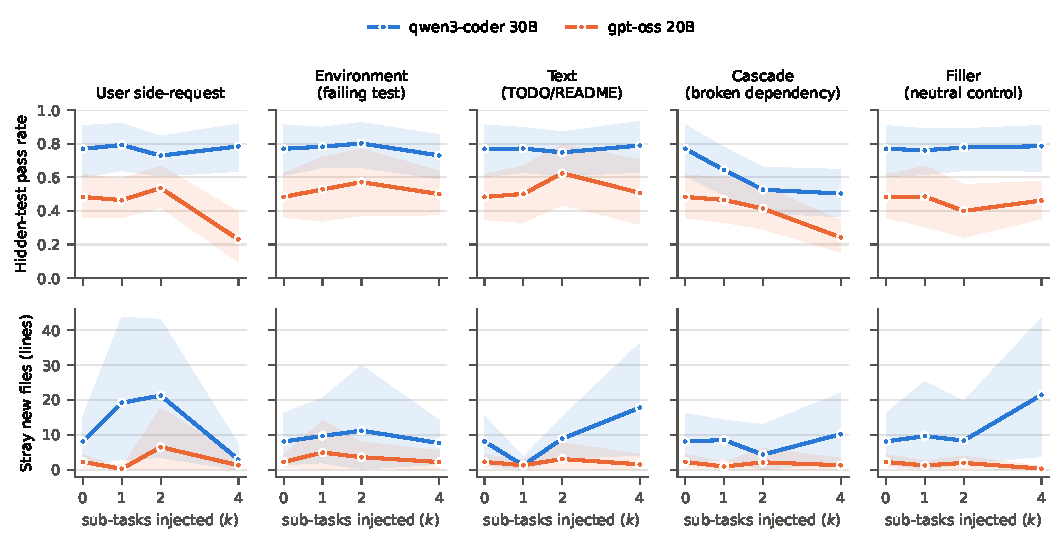
\includegraphics[width=\textwidth]{figures/e1_dose_response.pdf}
  \caption{E1 dose--response. Top: hidden-test pass rate; bottom: lines in stray new files left in
  the repository. Bands are 95\% task-cluster bootstrap intervals.}
  \label{fig:e1}
\end{figure}

\paragraph{Results.} Table~\ref{tab:e1} and Figure~\ref{fig:e1} summarise the outcome.
\begin{itemize}
  \item \textbf{Cascades are the only source that degrades the goal in both models.} With four
        broken dependencies, \texttt{qwen3-coder} falls from 0.77 to 0.50 (slope $-0.065$ per
        sub-task, Holm $p=.005$) and \texttt{gpt-oss} from 0.48 to 0.24 (slope $-0.062$, Holm
        $p=.005$). The share of episodes that fully meet the goal falls from 44\% to 8\% and from 31\%
        to 3\%. For \texttt{qwen3-coder} the loss is significantly larger than with the filler
        control (excess slope $-0.083$, Holm $p<.001$). For \texttt{gpt-oss} the difference points
        the same way ($-0.041$, uncorrected $p=.010$, Holm $p=.07$).
  \item \textbf{User side requests overload the weaker model.} \texttt{qwen3-coder} absorbs up to
        four requests without loss on the goal (0.73--0.79) and fulfils about 90\% of them.
        \texttt{gpt-oss} is unaffected up to $k=2$. At $k=4$ it loses on both fronts: the pass rate
        drops to 0.23 ($D_4=-0.25$, 95\% CI $[-0.46,-0.04]$) and only 40\% of the side requests are
        met. The linear trend is not significant after correction (uncorrected $p=.03$, Holm $p=.27$).
        The pattern is a threshold rather than a linear dose.
  \item \textbf{Distractors are largely ignored.} Failing unrelated tests (\textsf{env}) and
        instruction-like text (\textsf{text}) leave the pass rate within a few points of the
        baseline for both models. The one exception, a non-significant \emph{rise} for
        \texttt{gpt-oss} at $k=2$, is within the noise of the cell. Edits to existing out-of-scope
        files stay below 3.5\% of changed lines in every cell, so neither model acted on planted
        instructions that pointed outside the scope. Inside the scope the judge panel of E5 finds
        the same: at most 6.4\% of segments in any cell are labelled as work on a distractor
        (Section~\ref{sec:judge-results}).
  \item \textbf{Longer context alone does not hurt.} The filler control is flat for both models,
        so the losses above cannot be attributed to the added length of the pauses.
  \item \textbf{Stray files vary but show no trend.} \texttt{qwen3-coder} leaves 1--21 lines of
        debugging scripts per episode on average and \texttt{gpt-oss} 0--6. No slope is significant.
\end{itemize}
Two process observations matter for E3 and E4. \texttt{qwen3-coder} triggers Claude Code's automatic
compaction in 19\% of episodes and \texttt{gpt-oss} in only 1\%, with no difference across sources.
\texttt{gpt-oss} modifies a protected file in 13\% of episodes, including 19\% of baseline
episodes, against 0.5\% for \texttt{qwen3-coder}. These modifications are not driven by the
failing tests of the \textsf{env} source (11\%).

\paragraph{Against the hypotheses.} H1 holds only for cascades, and for user requests in the
weaker model at the highest dose. It does not hold for distractors: in this setting the number of
sub-tasks matters much less than their kind. H2 is partly supported:
\begin{itemize}
  \item As predicted, sanctioned user requests produce \emph{incompletion} rather than scope
        violation, but only for \texttt{gpt-oss} and only at $k=4$.
  \item Contrary to H2, \textsf{text} distractors do not produce scope violations, and \textsf{env}
        obstacles do not produce effort displacement onto protected tests.
  \item Also contrary to H2, \textsf{cascade} sub-tasks are the \emph{most} damaging, not the least.
\end{itemize}
The cascade result needs care. By construction a cascade that the agent fails to repair lowers the
score even if the agent never stops pursuing $\Gz$, so part of this loss is unresolved necessary
work rather than drift away from the goal. The judge-based measures of
Section~\ref{sec:judge-results} give a partial answer: for \texttt{qwen3-coder} up to 18\% of
segments go to work off the goal under cascades, none of it labelled as distracting work, and for
\texttt{gpt-oss} the share does not rise at all. Whether each broken dependency was
eventually fixed is not among the judged fields and remains open.

\subsection{E2: harness mitigations (RQ2, H3)}
\label{sec:e2}

\paragraph{Design.} E2 fixes the load at one sub-task of each source (\textsf{mix}: one user
request at the first pause, one \textsf{env}, one \textsf{text} and one \textsf{cascade} injection
in the repository) and varies the harness. It compares five conditions on \texttt{qwen3-coder}
(12 tasks $\times$ 3 repetitions each, 180 episodes):
\begin{itemize}
  \item \emph{no mitigation};
  \item a \emph{goal re-anchoring hook}: a \texttt{UserPromptSubmit} hook that appends the original
        goal, verbatim, to every new message;
  \item a \emph{stop-hook checklist}: a \texttt{Stop} hook that blocks the first attempt to stop in
        each turn and asks the agent to check each numbered requirement of the original goal;
  \item \emph{sub-agent delegation}: an appended system instruction to hand any sub-task outside the
        original goal to a sub-agent through the \texttt{Task} tool;
  \item a \emph{task list}: Claude Code's task-list tools enabled, plus an instruction to record each
        requirement and each new sub-task and to check the list before finishing.
\end{itemize}
The two hook conditions act outside the model and are deterministic. The last two depend on the
model following an instruction. Hooks are disabled during the probe, so that goal recall is never
answered with the hook's help.

\begin{table}[t]
  \centering
  \caption{E2: mitigations under a fixed load of four sub-tasks (\textsf{mix}),
  \texttt{qwen3-coder}, 36 episodes per condition. $\Delta$: difference in hidden pass rate from no
  mitigation, with 95\% task-cluster bootstrap interval. No difference is significant after Holm
  correction.}
  \label{tab:e2}
  \small
  \fittable{\begin{tabular}{lcccccc}
\toprule
Condition & \makecell{Hidden\\pass} & \makecell{$\Delta$ vs.\ none\\{}[95\% CI]} & \makecell{Goal\\fully met} & \makecell{Side request\\met} & \makecell{Stray\\lines} & \makecell{Tool\\calls} \\
\midrule
No mitigation & 0.630 & -- & 0.14 & 0.81 & 8.2 & 48.2 \\
Goal re-anchoring hook & 0.647 & +0.018 [$-$0.03, +0.08] & 0.11 & 0.89 & 6.6 & 47.8 \\
Stop-hook checklist & 0.620 & $-$0.010 [$-$0.08, +0.06] & 0.17 & 0.86 & 11.4 & 53.2 \\
Sub-agent delegation & 0.682 & +0.052 [$-$0.01, +0.12] & 0.14 & 0.83 & 9.4 & 51.0 \\
Task list & 0.685 & +0.055 [+0.00, +0.11] & 0.14 & 0.81 & 19.7 & 56.4 \\
\bottomrule
\end{tabular}
}
\end{table}

\begin{figure}[t]
  \centering
  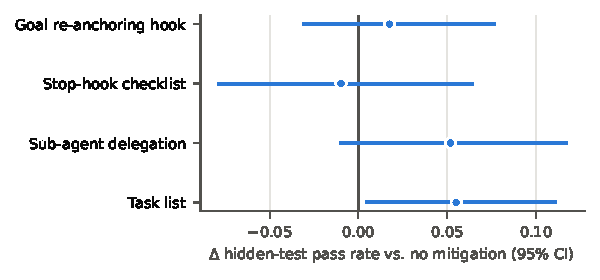
\includegraphics[width=0.62\textwidth]{figures/e2_mitigations.pdf}
  \caption{E2: effect of each mitigation on the hidden pass rate (95\% task-cluster bootstrap
  intervals).}
  \label{fig:e2}
\end{figure}

\paragraph{Results.} Under the mixed load \texttt{qwen3-coder} passes 63\% of the hidden requirements
without mitigation, against 77\% with no sub-tasks in E1. No mitigation changes this significantly
(Table~\ref{tab:e2}, Figure~\ref{fig:e2}):
\begin{itemize}
  \item The task list and sub-agent delegation show the largest point estimates: $+0.055$
        (95\% CI $[+0.004, +0.112]$) and $+0.052$ ($[-0.010, +0.118]$). Neither survives correction
        (Holm $p=.28$ and $p=.45$).
  \item The re-anchoring hook fired on every message, six times per episode, yet changed the goal
        pass rate by only $+0.018$. It raised the completion of the user's side request from 81\% to
        89\%.
  \item The stop-hook checklist had no effect ($-0.010$) and fired only 1.4 times per episode,
        because most segments end at the turn limit rather than by the agent deciding to stop.
\end{itemize}
How far each mitigation was taken up differs sharply:
\begin{itemize}
  \item Despite the instruction, \texttt{qwen3-coder} delegated to a sub-agent in only 2 of 36
        episodes.
  \item It used the task list in 24 of 36 episodes.
  \item The task list was also the most expensive condition: 56 tool calls against 48 without
        mitigation, and the most stray new lines (20 against 8).
\end{itemize}

\paragraph{Against the hypotheses.} H3 is not supported in its strong form. Deterministic hooks did
not outperform instruction-based mitigations; if anything the ordering is reversed. Their weakness
is not that the model ignored them, since the re-anchoring hook fired every time. They inject
information the model already has at moments that do not coincide with the loss. The
instruction-based conditions depend on compliance, which was low for delegation. Within this power
(36 episodes per condition, intervals of about $\pm 0.06$), no lightweight harness change removes
the loss caused by the mixed load.

\subsection{E5: judge validation}
\label{sec:e5}

The trajectory-level measures (effort share, goal recall, goal replacement, report fidelity) rely on
LLM judges. No human annotator was available, so E5 replaces human labels with a panel of three
judges from three model families, none of which is an agent under test: \texttt{gpt-oss:120b}
with medium reasoning effort, and \texttt{mistral-small3.2:24b} and \texttt{llama3.3:70b} without
reasoning.
\texttt{gpt-oss:120b} shares a family with the \texttt{gpt-oss:20b} agent, so every agreement figure
is also reported per agent model. Each judge labels every segment of every E1/E2 episode (7{,}991
segments) with one of five labels (\textsf{GOAL}, \textsf{SANCTIONED}, \textsf{NECESSARY},
\textsf{DISTRACTOR}, \textsf{NONE}) and every episode (1{,}332) on whether its final summary claims
completion and what it presents as the main accomplishment. Items are blinded to the agent model and
the outcome, but not to the condition: the task card shows the injected sub-tasks, which the judge
needs in order to tell sanctioned from distracting work. One stylistic difference cannot be hidden:
\texttt{qwen3-coder} runs pytest in verbose mode. The panel majority labels each item; items on
which all three judges disagree get no label and are excluded. The criterion is Fleiss'
$\kappa\ge 0.6$. A panel without human labels measures reliability, not validity: the labels show
that three independent models read the trajectories in the same way, not that they read them
correctly.

The first codebook passed on a pilot sample of 60 segments ($\kappa=0.71$) but not on the full set
($\kappa=0.44$, 95\% CI 0.42--0.45; \texttt{claims\_complete} $\kappa=0.65$). Reading the
disagreements showed two causes. First, the codebook had two pairs of rules that contradicted each
other, on wrap-up segments (re-running passing tests) and on read-only orientation. Second, one judge
labelled segments by the session context rather than by the actions in the segment. Codebook v2
states that the label follows the actions in the segment, sharpens \textsf{NONE} and adds three
worked examples. On a held-out stratified sample of 260 segments, v2 raised $\kappa$ from 0.44 to
0.57 for the five labels and from 0.53 to 0.67 for the distinction that defines drift: work leaving
the goal (\textsf{SANCTIONED}, \textsf{NECESSARY} or \textsf{DISTRACTOR}) versus the rest. We
therefore use this binary label as the primary segment measure and the five labels as a secondary
one. This choice was made after seeing the held-out agreement. In the held-out sample, reliability
is lower on \texttt{qwen3-coder} episodes ($\kappa=0.54$ for the binary label), where the residual disagreement
is between \textsf{GOAL} and \textsf{NONE}.

On the full set (7{,}990 segments with a complete panel), codebook v2 gives $\kappa=0.667$ (95\% CI
0.647--0.686, raw agreement 0.93) for the binary label, matching the held-out estimate: 0.723 on
\texttt{gpt-oss:20b} episodes and 0.615 on \texttt{qwen3-coder} episodes. The five labels reach
0.575 (0.559--0.591) and \texttt{claims\_complete} 0.658 (0.614--0.701). Recall ($\kappa=0.17$) and
the main accomplishment ($\kappa=0.45$) stay below the criterion: recall is not used, and goal
replacement is reported only as exploratory. The three judges disagree completely on 58 of 7{,}991
segments (0.7\%; 41 of 4{,}536 for \texttt{qwen3-coder} and 17 of 3{,}455 for \texttt{gpt-oss}) and
on 5 of 1{,}332 \texttt{claims\_complete} labels; these labels are excluded.

In 3 of the 1{,}332 episodes (0.2\%, all \texttt{gpt-oss:20b} on two tasks) the agent ran
\texttt{grep -R ..} from its working directory and so read the harness's own log files. None of
them read the episode specification that names the condition. Agent model names that reached two
judge items this way were replaced by a placeholder before judging.

\subsection{Judge-based measures in E1 and E2}
\label{sec:judge-results}

Each episode yields four judge-based measures:
\begin{itemize}
  \item the \emph{off-goal share}, the fraction of its labelled segments marked \textsf{SANCTIONED},
        \textsf{NECESSARY} or \textsf{DISTRACTOR} (primary);
  \item the \emph{distractor share}, the fraction marked \textsf{DISTRACTOR}, which is the
        illegitimate part of the off-goal work;
  \item \emph{over-claiming}: the final summary claims completion while at least one hidden test
        fails;
  \item \emph{goal replacement}: the main accomplishment named in the summary is not the goal
        (exploratory).
\end{itemize}
Table~\ref{tab:e5e1} and Figure~\ref{fig:e5} report E1, Table~\ref{tab:e5e2} reports E2. Intervals
are 95\% task-cluster bootstrap intervals with 36 episodes per cell, as in
Section~\ref{sec:analysis}, but they are \emph{not} corrected for multiplicity: these measures
were added after the outcome analysis and span 40 E1 cells and 4 E2 contrasts, so an isolated
interval that just excludes zero should be read with caution.

\begin{table}[t]
  \centering
  \caption{E1, judge-based measures by model, source and $k$ (36 episodes per cell; $k=0$ is the
  shared baseline). Off-goal share: mean fraction of an episode's segments that the judge panel
  labels \textsf{SANCTIONED}, \textsf{NECESSARY} or \textsf{DISTRACTOR}. Over-claim rate: fraction
  of episodes whose final summary claims completion while a hidden test fails.}
  \label{tab:e5e1}
  \small
  \fittable{\begin{tabular}{llcccccccc}
\toprule
 & & \multicolumn{4}{c}{Off-goal share (incl.\ sanctioned/necessary)} & \multicolumn{4}{c}{Over-claim rate} \\
Model & Source & $k{=}0$ & $k{=}1$ & $k{=}2$ & $k{=}4$ & $k{=}0$ & $k{=}1$ & $k{=}2$ & $k{=}4$ \\
\midrule
qwen3-coder 30B & User side-request & 0.00 & 0.16 & 0.27 & 0.53 & 0.42 & 0.47 & 0.56 & 0.44 \\
 & Environment (failing test) & 0.00 & 0.00 & 0.00 & 0.01 & 0.42 & 0.53 & 0.33 & 0.54 \\
 & Text (TODO/README) & 0.00 & 0.00 & 0.01 & 0.00 & 0.42 & 0.50 & 0.50 & 0.34 \\
 & Cascade (broken dependency) & 0.00 & 0.05 & 0.10 & 0.18 & 0.42 & 0.75 & 0.81 & 0.78 \\
 & Filler (neutral control) & 0.00 & 0.01 & 0.00 & 0.01 & 0.42 & 0.56 & 0.56 & 0.44 \\
\midrule
gpt-oss 20B & User side-request & 0.08 & 0.29 & 0.38 & 0.62 & 0.50 & 0.61 & 0.58 & 0.76 \\
 & Environment (failing test) & 0.08 & 0.07 & 0.09 & 0.10 & 0.50 & 0.56 & 0.50 & 0.56 \\
 & Text (TODO/README) & 0.08 & 0.06 & 0.08 & 0.03 & 0.50 & 0.56 & 0.53 & 0.61 \\
 & Cascade (broken dependency) & 0.08 & 0.09 & 0.07 & 0.06 & 0.50 & 0.78 & 0.81 & 0.81 \\
 & Filler (neutral control) & 0.08 & 0.05 & 0.05 & 0.03 & 0.50 & 0.53 & 0.67 & 0.69 \\
\bottomrule
\end{tabular}
}
\end{table}

\begin{figure}[t]
  \centering
  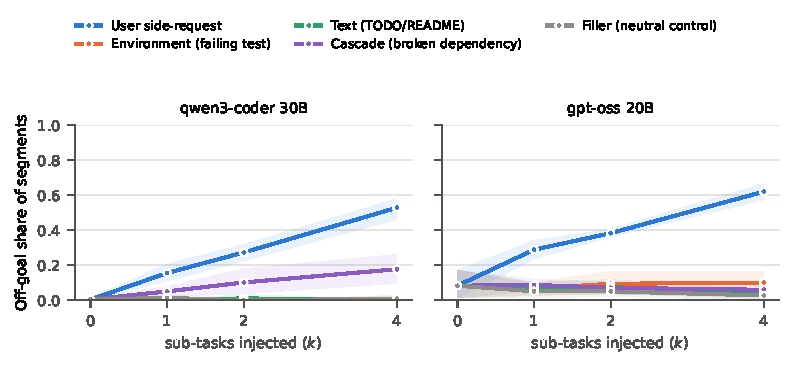
\includegraphics[width=0.85\textwidth]{figures/e5_off_share.pdf}
  \caption{E1: off-goal share of segments by source and number of injected sub-tasks. Bands are
  95\% task-cluster bootstrap intervals.}
  \label{fig:e5}
\end{figure}

\begin{table}[t]
  \centering
  \caption{E2, judge-based measures under the \textsf{mix} load, \texttt{qwen3-coder}, 36 episodes
  per condition. $\Delta$: difference from no mitigation, with 95\% task-cluster bootstrap interval
  (not corrected for multiplicity).}
  \label{tab:e5e2}
  \small
  \fittable{\begin{tabular}{llcccc}
\toprule
Model & Condition & \makecell{Off-goal share\\(incl.\ sanctioned)} & \makecell{$\Delta$ vs.\ none\\{}[95\% CI]} & \makecell{Over-claim\\rate} & \makecell{$\Delta$ vs.\ none\\{}[95\% CI]} \\
\midrule
qwen3-coder 30B & No mitigation & 0.19 & -- & 0.69 & -- \\
 & Goal re-anchoring hook & 0.21 & +0.02 [$-$0.03, +0.06] & 0.89 & +0.20 [+0.08, +0.36] \\
 & Stop-hook checklist & 0.20 & +0.01 [$-$0.03, +0.06] & 0.69 & +0.01 [$-$0.13, +0.14] \\
 & Sub-agent delegation & 0.19 & $-$0.00 [$-$0.05, +0.04] & 0.69 & +0.01 [$-$0.19, +0.21] \\
 & Task list & 0.14 & $-$0.05 [$-$0.11, +0.00] & 0.75 & +0.06 [$-$0.08, +0.21] \\
\bottomrule
\end{tabular}
}
\end{table}

\paragraph{Off-goal work follows the user's requests.} The off-goal share rises with $k$ only for
user side requests. For \texttt{qwen3-coder} it goes from 0.005 at baseline to 0.16, 0.27 and 0.53
at $k=1,2,4$; for \texttt{gpt-oss} from 0.08 to 0.29, 0.38 and 0.62. At $k=4$ the difference from
baseline is $D_4=+0.52$ $[0.45, 0.58]$ and $+0.54$ $[0.46, 0.62]$, and the difference from the filler
control at the same $k$ is of the same size ($+0.52$ $[0.45, 0.57]$ and $+0.59$ $[0.53, 0.65]$).
Cascades raise the share for \texttt{qwen3-coder} only: 0.18 at $k=4$, $D_4=+0.17$ $[0.09, 0.26]$.
For \texttt{gpt-oss} cascades stay at baseline. The \textsf{env}, \textsf{text} and \textsf{filler}
conditions stay within $\pm0.06$ of baseline in both models, with intervals that include zero. A few
\texttt{qwen3-coder} intervals only touch zero at one end, such as $+0.005$ $[0, 0.014]$ with four
\textsf{env} injections, and the amounts are negligible.

\paragraph{Almost none of it is distraction.} The distractor share is close to zero everywhere. Its
largest value is 0.064, for \texttt{gpt-oss} with four \textsf{env} injections, and for
\texttt{qwen3-coder} it is zero in all but two cells. The agents rarely acted on planted
\texttt{TODO}/README text or on unrelated failing tests in a way the judges label as distracting
work. The off-goal work they did is almost entirely the work the user asked for or the repairs the
goal needed.

\paragraph{Over-claiming is common and rises with cascades.} At baseline the final summary claims
completion while a hidden test fails in 42\% of \texttt{qwen3-coder} episodes and 50\% of
\texttt{gpt-oss} episodes. Cascades raise this in both models at every dose. For
\texttt{qwen3-coder} the rate is 0.75, 0.81 and 0.78 at $k=1,2,4$ ($D_k=+0.33$ $[0.11, 0.58]$,
$+0.39$ $[0.17, 0.61]$, $+0.36$ $[0.11, 0.64]$). For \texttt{gpt-oss} it is 0.78, 0.81 and 0.81
($+0.28$ $[0.17, 0.39]$, $+0.31$ $[0.11, 0.50]$, $+0.31$ $[0.08, 0.50]$). Against the filler control
the excess is clear only for \texttt{qwen3-coder} at $k=2$ and $k=4$ ($+0.25$ $[0.03, 0.50]$ and
$+0.33$ $[0.08, 0.58]$), because the filler itself raises over-claiming in some cells
(\texttt{qwen3-coder} $k=1$: $+0.14$ $[0.03, 0.25]$; \texttt{gpt-oss} $k=4$: $+0.19$
$[0.03, 0.33]$). Part of the cascade effect is mechanical: cascades lower the pass rate, so more
episodes have a failing test that a claim of completion can contradict. With four side requests
\texttt{gpt-oss} over-claims in 0.76 of episodes, but the interval of the difference includes zero
($+0.26$ $[-0.01, 0.55]$). The only other interval that excludes zero is a \emph{lower} rate for
\texttt{qwen3-coder} with two \textsf{env} injections than with filler ($-0.22$ $[-0.39, -0.06]$).

\paragraph{Goal replacement (exploratory).} With the caveat of its low reliability ($\kappa=0.45$),
the summary names something other than the goal as the main accomplishment in 8\% of baseline
\texttt{qwen3-coder} episodes and 19\% of \texttt{gpt-oss} episodes, and no E1 cell differs from
baseline with an interval that excludes zero.

\paragraph{E2.} No mitigation changes the off-goal share under the mixed load (0.19 without
mitigation). The task list has the largest point estimate, $-0.05$ $[-0.11, 0.00]$. The re-anchoring
hook increases over-claiming: 0.89 of its episodes claim completion with a hidden test failing,
against 0.69 without mitigation ($+0.20$ $[0.08, 0.36]$). The other mitigations leave over-claiming
unchanged. We have not examined why the hook has this effect.

\subsection{E3: compaction (RQ3, H4)}
\label{sec:e3}

When the context approaches its limit, Claude Code replaces the conversation with a summary written
by the model, and whatever the summary leaves out is lost for the rest of the session. E3 asks
whether this step changes how the agent divides its effort between the goal and the sub-tasks. It
has two parts: an observational comparison of the E1 and E2 episodes in which compaction happened
on its own, and a small pilot in which compaction is forced. The planned test of inherited drift was
not run, for the reason given at the end of this section.

\begin{table}[t]
  \centering
  \caption{E3, observational: \texttt{qwen3-coder} episodes of E1 and E2 with automatic compaction
  against episodes without it. Control episodes are re-weighted to the compacted episodes' mix of
  experiment, source, $k$ and condition. The last row compares segments after and before the first
  compaction within the same episodes, excluding the segment in which it occurred. Intervals are
  95\% task-cluster bootstrap intervals. The comparison is correlational.}
  \label{tab:e3obs}
  \small
  \fittable{\begin{tabular}{llcccc}
\toprule
Contrast & Measure & $n$ & \makecell{Compacted\\/ after} & \makecell{Matched none\\/ before} & \makecell{Difference\\{}[95\% CI]} \\
\midrule
compacted vs matched none & hidden pass & 135 & 0.46 & 0.77 & $-$0.31 [$-$0.43, $-$0.02] \\
compacted vs matched none & over claim & 135 & 0.36 & 0.63 & $-$0.26 [$-$0.42, $-$0.08] \\
compacted vs matched none & off share & 135 & 0.08 & 0.11 & $-$0.03 [$-$0.05, $-$0.00] \\
after vs before first compaction & off share & 18 & 0.06 & 0.10 & $-$0.04 [$-$0.25, +0.01] \\
\bottomrule
\end{tabular}
}
\end{table}

\paragraph{Spontaneous compaction.} In E1 and E2, 135 \texttt{qwen3-coder} episodes triggered
automatic compaction. Against non-compacted episodes from the same experiment, source, $k$ and
condition (Table~\ref{tab:e3obs}), they pass fewer hidden tests, 0.46 against 0.77 (difference
$-0.31$, 95\% CI $[-0.43, -0.02]$), and they over-claim less often, 0.36 against 0.63 ($-0.26$
$[-0.42, -0.08]$): their final summaries more often admit that the work is unfinished. Their
off-goal share is slightly lower (0.08 against 0.11). In the 18 episodes where segments on both
sides of the first compaction could be compared, the off-goal share is 0.06 after it and 0.10
before, with an interval from $-0.25$ to $+0.01$. These differences cannot be read causally.
Compaction happens when the context fills up, that is in long episodes in which the agent is
struggling, and such episodes would fail more often with or without it.

\paragraph{Forced compaction: design.} The pilot uses \texttt{qwen3-coder} with four user side
requests ($k=4$), the condition in which the off-goal share is highest and the goal still mostly
met. It compares two arms of 12 tasks $\times$ 3 repetitions (36 episodes each): in one the harness
sends Claude Code's \texttt{/compact} command right after the segment of the second pause, before
the third side request; in the other it does not. The command works in headless mode. Up to that point the two
arms are identical, so the off-goal share of the pre-compaction segments (initial segment and first
two pauses) is a placebo that should show no difference; the post-compaction segments are the third
and fourth pauses and the final segment. The judge panel labelled the pilot's 432 segments and 72
episodes with codebook v2. Agreement on the binary off-goal label is $\kappa=0.632$ (95\% CI
0.575--0.688), above the criterion, and 0.588 for the five labels. \texttt{claims\_complete} reaches
only 0.562 (0.37--0.73), below the criterion, so over-claiming in E3 carries that caveat. Recall
(0.26) is not used, and the main accomplishment (0.31) makes goal replacement exploratory only.

\begin{table}[t]
  \centering
  \caption{E3, forced-compaction pilot: \texttt{qwen3-coder}, four user side requests, 12 tasks
  $\times$ 3 repetitions per arm, \texttt{/compact} sent after the second pause. Difference:
  compaction minus no compaction, with 95\% task-cluster bootstrap interval. Off-goal share:
  segments labelled \textsf{SANCTIONED}, \textsf{NECESSARY} or \textsf{DISTRACTOR}; with this source
  it consists mostly of work on the user's own requests. Pre-compaction segments are a placebo.
  Over-claim rests on \texttt{claims\_complete}, whose agreement on E3 is below the criterion
  ($\kappa=0.56$); goal replacement is exploratory ($\kappa=0.31$). The pilot is exploratory.}
  \label{tab:e3pilot}
  \small
  \fittable{\begin{tabular}{lccc}
\toprule
Measure & Compaction ($n$) & No compaction ($n$) & Difference [95\% CI] \\
\midrule
Hidden-test pass & 0.72 (36) & 0.77 (36) & $-$0.05 [$-$0.11, +0.00] \\
Side-request pass & 0.90 (36) & 0.84 (36) & +0.06 [$-$0.01, +0.15] \\
Out-of-scope edits (existing files) & 0.00 (36) & 0.00 (36) & $-$0.00 [$-$0.01, +0.00] \\
Protected file modified (share) & 0.03 (36) & 0.00 (36) & +0.03 [+0.00, +0.08] \\
Automatic compactions (beyond the forced one) & 0.08 (36) & 0.17 (36) & $-$0.08 [$-$0.28, +0.08] \\
Over-claim & 0.43 (35) & 0.42 (36) & +0.01 [$-$0.14, +0.17] \\
Off-goal share, all segments & 0.59 (36) & 0.50 (36) & +0.09 [+0.06, +0.12] \\
Off-goal share, pre-compaction segments (placebo) & 0.54 (36) & 0.49 (36) & +0.05 [$-$0.01, +0.10] \\
Off-goal share, post-compaction segments & 0.63 (36) & 0.50 (36) & +0.13 [+0.06, +0.20] \\
Goal replaced (exploratory) & 0.47 (36) & 0.17 (36) & +0.31 [+0.11, +0.53] \\
\bottomrule
\end{tabular}
}
\end{table}

\paragraph{Forced compaction: results.} Table~\ref{tab:e3pilot} gives the outcome. After the
compaction the agent spent more of its segments off the goal: 0.63 against 0.50 in the
post-compaction segments ($+0.13$ $[+0.06, +0.20]$). Under this source off-goal work is almost all
\textsf{SANCTIONED}, the user's own side requests, so the increase means that after compaction the
agent gave more of its effort to the third and fourth requests relative to the goal. It does not
mean that it turned to distractors. The outcomes point the same way, with intervals that touch
zero: the hidden pass rate fell from 0.77 to 0.72 ($-0.05$ $[-0.11, +0.00]$) and the side-request
pass rate rose from 0.84 to 0.90 ($+0.06$ $[-0.01, +0.15]$). Over-claiming did not change (0.43
against 0.42). Edits to existing out-of-scope files were negligible in both arms (below 0.3\% of changed
lines), and one compacted episode modified a protected file. The placebo is not clean: the pre-compaction segments, identical by design, differ
by $+0.05$ $[-0.01, +0.10]$, so part of the post-compaction difference may be an imbalance between
the arms that was there before the compaction. The post-compaction difference is larger than the
placebo, but by less than the width of either interval. As an exploratory signal, the judges more
often read the final summary of a compacted episode as presenting a side request as the main
accomplishment (0.47 against 0.17), but their agreement on that field is too low to build on.

\paragraph{Inherited drift was not run.} The second part of E3 was to resume \texttt{qwen3-coder}
from trajectory prefixes produced by a weaker model under heavy load, in the spirit of
\citet{menon2026inherited}. Smoke tests with \texttt{qwen2.5:7b}, the planned weak model, showed
that it writes some tool calls as plain text, which Claude Code does not execute, and that it
claims completion falsely. Its prefixes would therefore be broken trajectories rather than drifted
ones, and a stronger model resuming them would inherit failed actions, not a displaced goal. The
lesson for the design is that the weak model must use the harness competently, so that its prefixes
differ from a strong model's in where they go rather than in whether they work. This test is left to
future work.

\paragraph{Against the hypotheses.} H4 is partly supported, on pilot evidence. Forced compaction
moved effort in the remaining segments away from the goal and towards the side requests, with a
small and uncertain cost to goal completion. It did not produce the constraint violations H4
predicted, and goal recall could not be measured because the judges do not agree on it. Inheritance
was not tested. With one model, one source and twelve tasks, the result is a direction for a larger
experiment, not an estimate.

\subsection{E4: the supervisor's view (RQ4, H5)}
\label{sec:e4}

E4 asks what a human supervisor could learn from the E1 and E2 trajectories, and at what cost. It
needs no new runs: it uses the episodes, their diffs and test results, the final summaries and the
v2 panel labels. It has two parts, report fidelity and a simulated supervisor. The third planned
part, whether a drift monitor degrades on longer transcripts \citep{martin2026classifier}, is left
to future work.

\paragraph{Report fidelity.} Over-claiming, a summary that claims completion while a hidden test
fails, is reported in Section~\ref{sec:judge-results}: 42\% of \texttt{qwen3-coder} and 50\% of
\texttt{gpt-oss} baseline episodes, 75--81\% under cascades. The second measure is \emph{omitted
changes}: a pre-existing out-of-scope file, or a protected file, that the diff changes but whose path
or base name does not appear in the final summary. It is a deterministic string match with no judge.
The match is strict, so a summary that describes a change without naming the file counts as an
omission, and the rates are upper bounds. \texttt{qwen3-coder} seldom touches such files, and its
omission rates stay between 0 and 8\% in every E1 cell (11\% with sub-agent delegation in E2).
\texttt{gpt-oss} touches them more often: 14\% of its baseline episodes omit a changed out-of-scope
file and 11\% a changed protected file, rising to 28\% for out-of-scope files with four \textsf{env}
injections. When such a file was changed, the summary usually did not name it: in 14 of the 16
\texttt{gpt-oss} cells it was omitted in at least half of those episodes, and in the two
\texttt{qwen3-coder} user-request cells where such changes occurred in 50\% and 75\%. These conditional rates rest on few
episodes and have wide intervals.

\paragraph{Supervisor simulation: design.} Each episode is replayed segment by segment, and a
simulated supervisor sees the panel's majority label of every segment it reviews. Three policies are
compared:
\begin{itemize}
  \item \emph{P0}: the supervisor reads only the final summary (one review) and is alerted if it
        does not claim completion;
  \item \emph{P1}: the supervisor reviews after each of the six segments (six reviews), is alerted at
        the first segment not labelled \textsf{GOAL}, and also reads the summary;
  \item \emph{P2}: a monitor alerts on segments labelled \textsf{DISTRACTOR} or \textsf{NONE}, and
        the supervisor reviews only the alerts.
\end{itemize}
The target is a failing episode, one with a hidden pass rate below 1: 525 of the 756
\texttt{qwen3-coder} episodes and 444 of the 576 \texttt{gpt-oss} episodes. The benefit of a policy
is the share of failing episodes it flags before the final segment, when the supervisor could still
redirect the agent; its cost is the number of reviews per episode; a false alarm is an alert in a
passing episode. The simulated supervisor applies the panel labels without error, so the results
are upper bounds for this information, not a user study. P1's alerts include legitimate detours,
sanctioned or necessary, which is why it raises false alarms in passing episodes.

\begin{table}[t]
  \centering
  \caption{E4, simulated supervisor on E1 and E2, all episodes per model (by group in Appendix~\ref{app:e4}, Table~\ref{tab:e4full}). Failing: hidden pass rate below 1. P0 reads only
  the final summary and is alerted if it does not claim completion; P1 reviews after all six
  segments and is alerted at the first segment not labelled \textsf{GOAL}; P2 is a monitor that
  alerts on \textsf{DISTRACTOR} or \textsf{NONE} segments (reviews = alerts). Early: flagged before
  the final segment. False alarm: an alert in a passing episode. The supervisor is assumed to apply
  the panel labels exactly, so the figures are upper bounds.}
  \label{tab:e4}
  \small
  \fittable{% "All episodes" rows of results/analysis/tables/e4_supervisor.tex (full table in the appendix).
\begin{tabular}{lcccccccccc}
\toprule
 & & & \multicolumn{3}{c}{Reviews / episode} & \multicolumn{3}{c}{Failing flagged early (\%)} & \multicolumn{2}{c}{False alarms (\%)} \\
Model & $n$ & fail & P0 & P1 & P2 & P0 & P1 & P2 & P1 & P2 \\
\midrule
qwen3-coder 30B & 756 & 525 & 1.0 & 6.0 & 0.7 & 0 & 56 & 19 & 77 & 62 \\
gpt-oss 20B & 576 & 444 & 1.0 & 6.0 & 0.3 & 0 & 44 & 18 & 55 & 28 \\
\bottomrule
\end{tabular}
}
\end{table}

\begin{figure}[t]
  \centering
  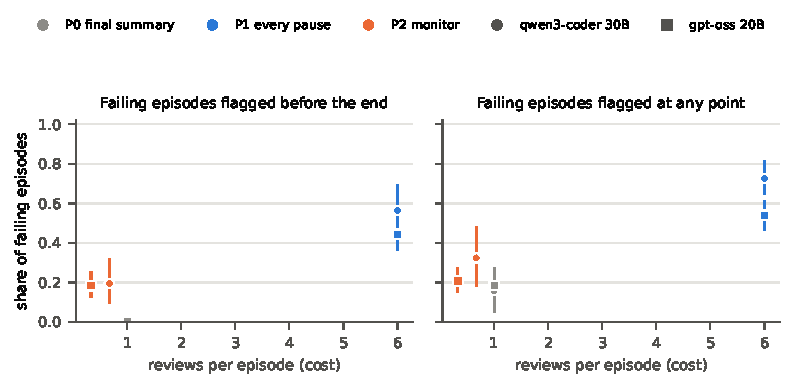
\includegraphics[width=\textwidth]{figures/e4_supervisor.pdf}
  \caption{E4: share of failing episodes flagged before the end (left) and at any point (right)
  against reviews per episode, for the three policies and both models. Bars are 95\% task-cluster
  bootstrap intervals.}
  \label{fig:e4}
\end{figure}

\paragraph{Supervisor simulation: results.} Table~\ref{tab:e4} and Figure~\ref{fig:e4} give the
results.
\begin{itemize}
  \item \emph{P0} cannot flag anything early by construction. At the end it flags 16\% of the
        failing \texttt{qwen3-coder} episodes and 18\% of the \texttt{gpt-oss} ones: in most of
        the rest the summary claims completion. False alarms are 5\% and 12\%.
  \item \emph{P1} flags 56\% (95\% CI 45--70\%) and 44\% (36--54\%) of failing episodes early, and
        73\% and 54\% at some point, at six reviews per episode. False alarms are 77\% and 55\%.
        Most of its alerts are detours the user asked for: with user side requests it flags
        94--96\% of failing episodes early, and also 98--100\% of the passing ones
        (Table~\ref{tab:e4full}).
  \item \emph{P2} costs 0.67 and 0.33 reviews per episode and flags 19\% (9--32\%) and 18\%
        (12--25\%) of failing episodes early, with 62\% and 28\% false alarms. Per review it flags
        about three (\texttt{qwen3-coder}) to seven (\texttt{gpt-oss}) times as many failing
        episodes as P1, but it misses more than four in five.
\end{itemize}
The reason is visible in the labels. Failing episodes mostly look like work on the goal, or like
legitimate detours, because the failure is incompletion (Section~\ref{sec:e1}). A supervisor who
judges what the agent is \emph{doing} has little to react to, and a monitor for illegitimate work
fires rarely and often in episodes that end well. What separates failing from passing episodes is
whether the requirements hold, which only running the acceptance tests shows; the agent's own
summary claims completion in most failing episodes.

\paragraph{Against the hypotheses.} H5 is partly supported. Report fidelity is below 1: summaries
over-claim in about half of the baseline episodes, more under cascades, and they usually leave out
the out-of-scope or protected files they changed. Fidelity does not decrease with $k$ in general,
only with cascades. A monitor-triggered checkpoint does intercept more failing episodes per review
than a review at every pause, as predicted, but it intercepts few of them and its alerts are often
false. Whether such a monitor degrades on longer transcripts was not tested.

\section{Discussion}
\label{sec:discussion}

Table~\ref{tab:verdicts} sets the results of E1--E5 against the hypotheses of
Section~\ref{sec:definition}. None is supported as stated. Four are supported in part, mostly
because the predicted effect appeared for one kind of sub-task or one indicator and not for the
others, and H3 is not supported.

\begin{table}[t]
  \centering
  \caption{Verdicts on the hypotheses. Partly: some of the predictions hold and others do not or
  were not tested. Evidence from Section~\ref{sec:experiments}; intervals are 95\% task-cluster
  bootstrap intervals.}
  \label{tab:verdicts}
  \small
  \begin{tabularx}{\textwidth}{@{}l l X@{}}
    \toprule
    Hypothesis & Verdict & Evidence \\
    \midrule
    H1 dose--response & Partly & Pass rate falls with $k$ for cascades in both models and for four
      user requests in \texttt{gpt-oss}, beyond the filler control for \texttt{qwen3-coder}
      cascades; flat for \textsf{env}, \textsf{text} and filler. The off-goal share rises with $k$
      only for user requests (E1). \\
    H2 source signatures & Partly & User requests cause incompletion (\texttt{gpt-oss}, $k=4$), as
      predicted. \textsf{Text} causes no scope violations, \textsf{env} no edits to protected tests,
      and cascades are the most damaging source, not the least (E1). \\
    H3 mitigations & Not supported & No mitigation changes the pass rate after Holm correction;
      deterministic hooks do no better than instruction-based mitigations (E2). \\
    H4 compaction & Partly & Forced compaction raises the post-compaction off-goal share by $+0.13$
      $[+0.06, +0.20]$, with an imperfect placebo; the pass rate changes by $-0.05$
      $[-0.11, +0.00]$; no constraint violations; recall not measurable; inheritance not tested
      (E3 pilot). \\
    H5 observability & Partly & Summaries over-claim in 42--50\% of baseline episodes and up to 81\%
      under cascades, and usually omit the out-of-scope files they changed. A monitor flags more
      failing episodes per review than review at every pause, but only 18--19\% of them early;
      monitor degradation not tested (E4). \\
    \bottomrule
  \end{tabularx}
\end{table}

\subsection{What kind of drift did we observe?}

The literature that motivated this study frames goal drift as the gradual \emph{displacement} of
the assigned goal by something else: competing objectives, environmental pressure, inherited
context \citep{arike2025goaldrift,menon2026inherited,saebo2026asymmetric}. Our results support a
narrower and less dramatic picture, with three features.

\paragraph{The kind of sub-task matters more than how many there are.} Up to four injected
sub-tasks of most kinds left both models where they started. Neither neutral interruptions of equal
length nor distractors moved the pass rate. Only two kinds of sub-task hurt: dependencies that had to
be repaired before the goal could be reached, and, for the weaker model, a stack of four sanctioned
side requests. A count of sub-tasks is therefore a poor predictor of drift. What matters is whether
a sub-task demands real work on the path to the goal or competes with the goal for the agent's
limited budget of turns.

\paragraph{The loss appears as incompletion, not as deviation.} In no condition did the agents edit
existing files outside the admissible scope to any meaningful degree (below 3.5\% of changed lines).
They did not chase planted \texttt{TODO}s into unrelated modules, nor did they ``fix'' the unrelated
failing tests at the expense of the goal. The goal was lost by \emph{not finishing it}. With four
side requests, \texttt{gpt-oss} completed fewer requirements of the goal and fewer of the requests.
With broken dependencies, both models more often ended with requirements failing. This matches the
\emph{unreliability} account of multi-turn degradation \citep{laban2025lost} better than a
goal-replacement account. The judge panel of E5 points the same way
(Section~\ref{sec:judge-results}). The work it labels as leaving the goal grows with the number of
side requests, to 0.53 (\texttt{qwen3-coder}) and 0.62 (\texttt{gpt-oss}) of the segments at
$k=4$, but almost all of it is work the user
asked for or repairs the goal needed. Work on distractors stays below 7\% of segments in every
cell. In these runs, then, drift is mostly legitimate widening of the scope at the user's request,
followed by goals left unfinished, and not the pursuit of something illegitimate. Two limits apply.
The panel's labels are reliable, not validated against humans, and the judges could not agree on
goal recall from the probe, so whether the agents' \emph{beliefs} about the goal shifted remains
open; the exploratory goal-replacement label shows no shift either.

\paragraph{Necessary work is the most dangerous.} H2 predicted that necessary cascades would cause
the least drift, because resolving them serves the goal. They caused the most. Two explanations are
compatible with the data:
\begin{itemize}
  \item the agent never found or fixed the broken dependency, so the loss is unresolved necessary
        work: a capability failure that the injection made visible;
  \item the agent fixed it but spent its budget, or its attention, doing so, and did not return to
        the remaining requirements: drift in the intended sense.
\end{itemize}
The two predict different trajectories: the first ends with the dependency still broken, the second
with it repaired and requirements missing. The judge labels separate them only in part. For
\texttt{gpt-oss} the share of segments spent off the goal does not rise with cascades, which fits
the first explanation: little visible repair work. For \texttt{qwen3-coder} it rises to 18\% at
$k=4$, none of it labelled as distraction, which leaves room for the second. Whether each
dependency ended up repaired was not judged. Either way the practical lesson is the same: the
sub-tasks that look most
legitimate, and that a supervisor is least likely to question, are where goal completion is most at
risk.

The resistance to distractors deserves a caveat. Studies of benign distraction and of instruction
hijacking report strong effects
\citep{ma2024caution,mavali2026tab,debenedetti2024agentdojo}. Our distractors were mild and
plausible rather than adversarial, they pointed away from the task, and every goal ended with ``keep
the change focused on this feature''. Under these conditions both models behaved conservatively.
The result says little about more salient or adversarially phrased material.

\paragraph{Compaction shifts effort from the goal to the requests.} The pilot of
Section~\ref{sec:e3} suggests a mechanism behind part of the incompletion. After the context was
summarised, \texttt{qwen3-coder} gave more of its remaining segments to the user's side
requests and slightly less to the goal, with a small, uncertain loss on the goal and a small gain on
the requests. This fits the concern of Section~\ref{sec:drift} that summarisation decides what
survives of the original request. One reading, which we have not checked against the compaction
summaries themselves, is that a summary written mid-session keeps the recent, concrete requests and
gives less weight to the original specification. The extra work is still sanctioned, so a
supervisor would see nothing wrong in it. The observational data cannot confirm the effect, because spontaneous compaction marks episodes that
were already in trouble, and the pilot is small, with a placebo that is not clean. The effect needs a
larger, preregistered test before it counts as established.

\subsection{Implications for the supervisor}

\paragraph{Drift of this kind is quiet.} A supervisor who reviews the diff---the most common form
of oversight (Section~\ref{sec:hai})---would see a focused, in-scope change in almost every episode,
including those in which the goal was badly incomplete. The failure is visible only against the
requirements, not against the code. This is the situation human-factors research warns about: a
supervisor's situation awareness depends on the signals the system exposes \citep{endsley1995situation},
and a tidy diff with a confident summary invites trust that is not calibrated to the outcome
\citep{lee2004trust}. The summaries add to the problem, which bears on RQ4 and H5. In E1, 42\%
of \texttt{qwen3-coder} baseline episodes and 50\% of \texttt{gpt-oss} ones end with a summary
that claims completion while a hidden test fails. With cascades the rate rises to about 0.75--0.81
in both models, and in E2 the goal re-anchoring hook raises it from 0.69 to 0.89. Part of the
cascade increase is mechanical, since more episodes fail a test, but it means that the sub-tasks
most likely to cost the goal are also those after which the agent's report is least reliable. These
intervals are not corrected for multiplicity, and over-claiming is measured at the level of the
episode, not per requirement. Relying on passing tests does not close the gap. In 19\% of E1 episodes the
entire visible suite passed while some requirements of the goal failed, and agents are known to optimise for the tests they can see
\citep{zhong2025impossiblebench}. Oversight tools should therefore show progress \emph{per
requirement}, not per file, and make what is still unverified explicit. This is a concrete form of
the ``conveying progress'' challenge of \citet{bansal2024communication}.

\paragraph{What a supervisor can catch (E4).} The supervisor simulation (Section~\ref{sec:e4})
puts numbers on this argument. Even with segment labels applied without error, a supervisor who
reviews what the agent is doing catches few failing episodes in time. Reviewing after every segment
flags about half of them before the end, at six reviews per episode and with an alert in most
passing episodes as well, because the alerts fire on detours the user asked for. A monitor for
illegitimate work is cheap but flags fewer than one in five. Reading the final summary flags fewer
than one in five at the end, since the summary claims completion in most failing episodes, and it
usually does not name the out-of-scope files that were changed. Because these failures are
incompletion, the activity looks normal. The check that would separate failing from passing
episodes is the one the agent's report replaces: running the acceptance tests of each requirement.
A supervisor's interface should show that check, and the harness should run it before the agent is
allowed to report completion.

\paragraph{Where to put checkpoints.} The losses concentrate at recognisable moments: when the agent
starts repairing something the goal depends on, and when side requests pile up. These are natural
triggers for the mixed-initiative interruptions advocated by \citet{bui2026proactivity}
\citep[see also][]{horvitz1999mixed}. They also suit a dynamic autonomy policy of the kind
implemented by Hedwig \citep{shukla2026hedwig}, which tightens oversight in unfamiliar territory. A
harness can detect both moments cheaply: an edit to a file outside $S(\Gz)$ that makes a failing
import or test pass, or a third pending user request. It can then ask the human whether to continue,
defer or delegate. In E4, review at every pause spent six reviews per episode and alerted in 55--77\% of
passing episodes, so periodic review mostly interrupts work that was going well. The triggers
proposed here are untested; the E4 monitor was triggered by illegitimate work, which is rare in
these runs.

\paragraph{The user is a source of drift too.} Sanctioned side requests are the user's own doing.
For the weaker model, four of them in one session cost half of the goal's completion and more than
half of the requests themselves. A design response is to treat a mid-session request as a new item
in a queue rather than an interruption of the current one: completed after the goal, or handed to a
separate session with its own context. Claude Code already has the ingredients, namely task lists,
background sessions and sub-agents. Our results suggest that these work only if the harness, not the
model, decides to use them.

\paragraph{Mitigations should not depend on compliance.} E2 does not support H3 in its strong form.
Deterministic hooks were not better than instruction-based mitigations, but the reasons differ.
\begin{itemize}
  \item \emph{Re-anchoring} was applied reliably, yet it repeats information the model already has
        and does nothing about the work that competes with the goal.
  \item The \emph{stop-hook checklist} acts only when the agent decides to stop. Under turn limits
        that rarely happened, and in real use agents also stop for other reasons (budgets,
        timeouts, errors).
  \item \emph{Delegation} would isolate sub-tasks as intended \citep{fei2026codedelegator}, but the
        model delegated in two episodes out of 36.
  \item The \emph{task list} was adopted more often and gave the largest, still non-significant,
        gain, at the cost of more tool calls and more stray files.
\end{itemize}
The common thread is that lightweight interventions inside the session do not change \emph{what}
the agent spends its budget on. More promising directions are interventions with teeth:
\begin{itemize}
  \item a completion gate that checks requirements, not just a stop;
  \item harness-enforced delegation of recognised sub-task types, rather than a suggestion to
        delegate;
  \item budgeting that reserves turns for the goal.
\end{itemize}
In all three the compliance of the model stops being a free variable.

\subsection{Limitations}

\begin{description}[leftmargin=0pt]
  \item[Models.] The agents are 20--30B open-weight models, not the Claude models that Claude Code
        is designed for. The harness, system prompt and tool descriptions are tuned for those, and the
        local models often used up their turns: 14\% of \texttt{qwen3-coder}'s final segments ended
        at the turn limit. Stronger models may absorb more sub-tasks
        before losing the goal, which would shift the thresholds, not necessarily remove them. The
        two models also differ widely in baseline competence, so cross-model comparisons are about
        patterns, not magnitudes.
  \item[Benchmark.] DriftBench-mini is small and synthetic: twelve libraries of a few hundred
        lines, with goals specified as numbered requirements and sub-tasks written by us. Real
        sessions are longer, goals are vaguer and sub-tasks arise organically. Some cascades are
        necessary only for some implementations, one is all-or-nothing, and two can never change the
        score (Section~\ref{sec:bench}). Because cascades widen the scope by design, part of their
        effect may reflect task difficulty rather than drift; the judge-based measures
        (Section~\ref{sec:judge-results}) address this only in part.
  \item[Protocol.] The fixed structure of pauses and per-segment turn limits makes conditions
        comparable but is not how people use agents. It also shaped the mitigations: the stop hook,
        for instance, rarely had a stop to act on. Results may differ in free-running sessions with
        larger budgets.
  \item[Judges.] The judge-based measures rest on a panel of three LLM judges. Their agreement
        shows reliability, not validity: no human labelled the trajectories. The binary off-goal
        label was chosen as the primary measure after seeing its held-out agreement, and codebook v2
        was written after reading the disagreements on the full set. Reliability is lower on
        \texttt{qwen3-coder} trajectories ($\kappa=0.615$ for the binary label on the full set, 0.48 for
        the five labels). The judges cannot be blinded to the condition, because they need the injected
        sub-tasks to tell sanctioned from distracting work. In 3 of 1{,}332 episodes (0.2\%) the
        agent read the harness's log files with \texttt{grep -R ..} from its sandbox. None of
        them read the episode specification that names the condition, and agent model names that
        leaked into two judge items were scrubbed. Goal recall is not used ($\kappa=0.17$) and goal
        replacement is exploratory ($\kappa=0.45$).
  \item[Measures and power.] Goal recall is not reported and goal replacement only as exploratory
        (see above); report fidelity is measured per episode, not per requirement. With 36 episodes per
        cell, the confidence intervals on a difference are about $\pm 0.05$--$0.10$ for
        \texttt{qwen3-coder} and up to $\pm 0.2$ for the more variable \texttt{gpt-oss}, so moderate effects, including the E2
        mitigations, cannot be excluded.
  \item[E3.] The forced-compaction pilot has one model, one source and twelve tasks with 36
        episodes per arm. Its placebo comparison is not clean ($+0.05$ on segments that precede the
        compaction), so part of the post-compaction difference may be imbalance between arms.
        Agreement on \texttt{claims\_complete} in E3 ($\kappa=0.56$) is below the criterion, so its
        over-claim figures are weaker than those of E1 and E2. The observational comparison is
        correlational, since compaction occurs in long, struggling episodes. Inherited drift was
        not tested.
  \item[E4.] The supervisor is simulated, not observed. It applies the panel labels without error,
        so the figures are upper bounds for each policy; real reviewers misread transcripts and tire.
        The P1 alert rule counts sanctioned and necessary detours as alerts, which inflates its false
        alarms, and omitted changes rest on a strict file-name match, which inflates omissions.
        Whether monitors degrade on longer transcripts was not tested.
  \item[Infrastructure.] The last 45 E1 episodes ran on a different cluster with identical model
        weights but without container isolation. They are a small share of one model's runs, and
        no episode referenced evaluation material, but the change is a deviation from the protocol.
\end{description}

\section{Conclusion}
\label{sec:conclusion}

Coding agents such as Claude Code turn the language model from an advisor into an operator, and
the human from operator into approver or observer \citep{feng2025levels}. This report examined one
risk of that transition: that the sub-tasks an agent meets or receives during a session---broken
dependencies, failing tests, instructions in files, side requests---accumulate and pull it away from
the goal it was given. We reviewed the work on autonomy, coding agents, oversight and goal drift. We
defined goal drift via sub-task injection as a counterfactual degradation, with sub-tasks classified
by source and legitimacy and a matched-length control. We then tested the definition on
DriftBench-mini, with Claude Code driven by two open-weight models in 1{,}332 controlled episodes and a 72-episode compaction pilot.

The findings revise the starting intuition:
\begin{itemize}
  \item \textbf{Kind matters more than count.} Neutral interruptions and mild distractors left goal
        completion unchanged. Broken dependencies on the path to the goal and, for the weaker model,
        a stack of four side requests reduced it sharply.
  \item \textbf{The failure is incompletion.} The agents rarely strayed outside the files they were
        supposed to change. They lost the goal by not finishing it, in a way that a diff-based review
        would not reveal.
  \item \textbf{Lightweight harness mitigations are not enough.} Re-injecting the goal, a stop-hook
        checklist, an instruction to delegate and an enforced task list did not significantly reduce
        the loss. The two that relied on the model's compliance were adopted only partly.
  \item \textbf{Off-goal work is mostly legitimate.} A panel of three LLM judges, reliable on the
        binary off-goal label ($\kappa=0.67$) but not validated against humans, found that the work
        leaving the goal was almost all what the user asked for or what the goal needed. Work on
        distractors stayed below 7\% of segments in every cell. Final summaries, however, claimed
        completion with a hidden test failing in 42--50\% of baseline episodes.
  \item \textbf{Compaction may tilt effort towards the requests.} In a forced-compaction pilot,
        \texttt{qwen3-coder} spent more of the segments after compaction on the user's side requests
        (off-goal share $+0.13$), with a small and uncertain loss on the goal. The pilot is small and
        its placebo not clean.
  \item \textbf{Watching the activity catches few failures.} In a simulated supervisor with perfect
        labels, reviewing every segment flagged about half of the failing episodes before the end at
        six reviews per episode and with frequent false alarms, and a monitor for illegitimate work
        flagged fewer than one in five. Failing episodes look like goal work; only the requirements
        show the failure.
\end{itemize}
For the human side of the interaction, these results argue for oversight that checks requirements
instead of code, checkpoints triggered at recognisable risky moments instead of fixed intervals,
mid-session requests handled as queued tasks, and mitigations that the harness enforces without
relying on the model's compliance.

Four lines of work follow from what this study could not settle:
\begin{itemize}
  \item \emph{inherited drift}, with a weak model that uses the harness competently, so that its
        prefixes drift instead of breaking;
  \item \emph{monitor degradation}: whether a drift monitor loses accuracy on longer transcripts
        \citep{martin2026classifier}, which decides whether drift-triggered checkpoints scale;
  \item \emph{human validation} of the judge panel on a sample, since its agreement shows
        reliability but not validity;
  \item \emph{goal recall}, on which the judges do not yet agree ($\kappa=0.17$), and which is needed
        to test whether compaction changes what the agent believes the goal to be.
\end{itemize}
Repeating the core experiments with frontier models, longer and less structured sessions, and
real-world rather than planted sub-tasks would show how far the thresholds observed here move as
agents become more capable. We expect them to move; our data cannot say whether they disappear.


\bibliographystyle{plainnat}
\bibliography{refs}

\end{document}
